\documentclass[a4paper, 13pt]{article}
\usepackage[margin=0.7in]{geometry}
\usepackage{framed}
\usepackage{graphicx}
\usepackage{xcolor}
\usepackage{blindtext}
\usepackage{xcolor}
\usepackage{mdframed}
\usepackage{indentfirst}
\usepackage{graphicx}
\usepackage{subcaption}
\usepackage{hyperref}
\usepackage{verbatim}
\usepackage{amsmath}
\usepackage{titling}
\usepackage{titlesec}
\usepackage[brazil]{babel}
\definecolor{LightGray}{gray}{0.97}
\usepackage{minted}
\usepackage{xcolor}


\usepackage{biblatex}
\addbibresource{refs.tex}


\setminted[fortran]{
  framesep=2mm,
  baselinestretch=1.2,
  bgcolor=LightGray,
  fontsize=\footnotesize,
  linenos}
  \graphicspath{{../src/graficos/}}
\hypersetup{
  pdfauthor={Jefter Santiago},
  pdftitle={Projeto 6 - Dinâmica Molecular},
  pdfcreator={Jefter Santiago}, 
  pdflang={Portuguese},
  colorlinks=true,    % Color links instead of boxes
  linkcolor=blue,     % Color of internal links
  citecolor=green,    % Color of citation links
  urlcolor=blue,      % Color of URLs
}
\title{\color{blue}Projeto 6 - Dinâmica molecular}
\author{Jefter Santiago (12559016)}
%\date{Entrega: 01/06/2024}
\begin{document}
\maketitle
\section{Introdução}




Potencial de Lennard-Jonnes

\begin{equation}
    \mathcal{U}(\vec{r}) = 4 \epsilon \left[ \left(\frac{\sigma}{r} \right)^12 - \left(\frac{\sigma}{r}\right)^6 \right]
\end{equation}
\section{Tarefa A}

\begin{figure}[h!]
    \centering
    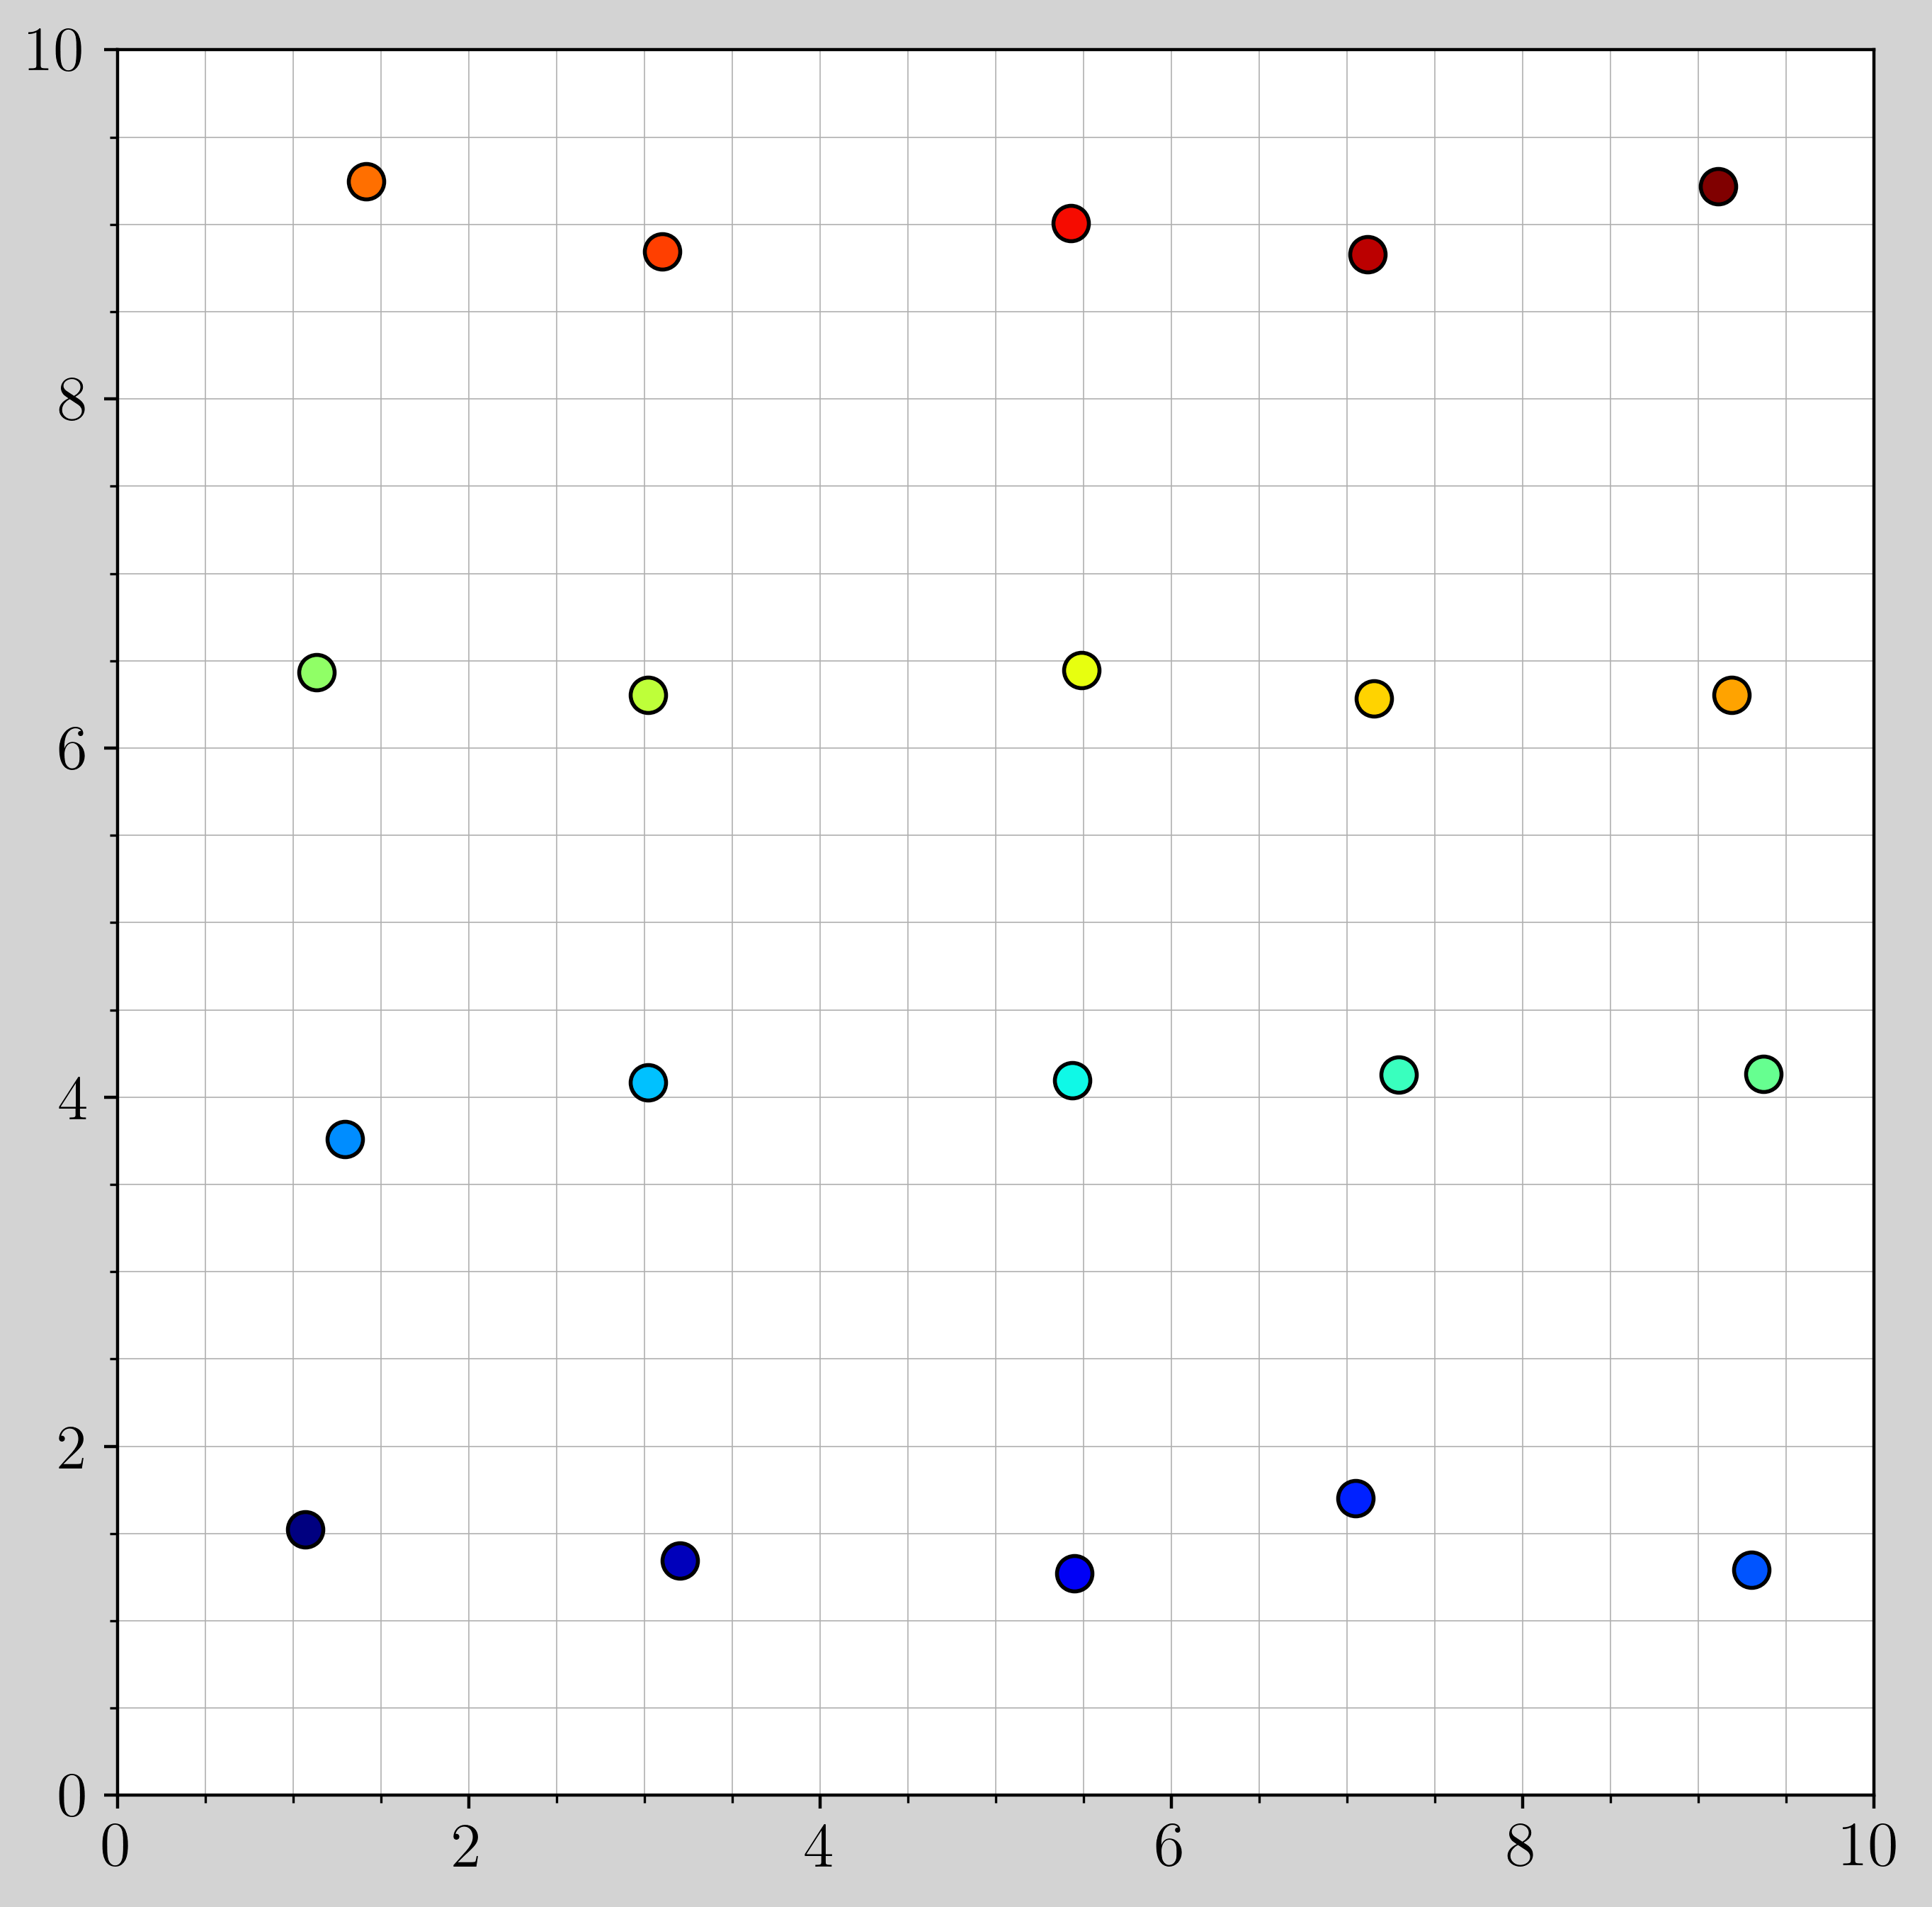
\includegraphics[width=0.4\linewidth]{tarefa-A/posicoes-iniciais.png}
    \caption{Posições iniciais das partículas.}
    \label{fig:posicoes-iniciais-a}
\end{figure}

\begin{figure}[h!]
    \centering 
    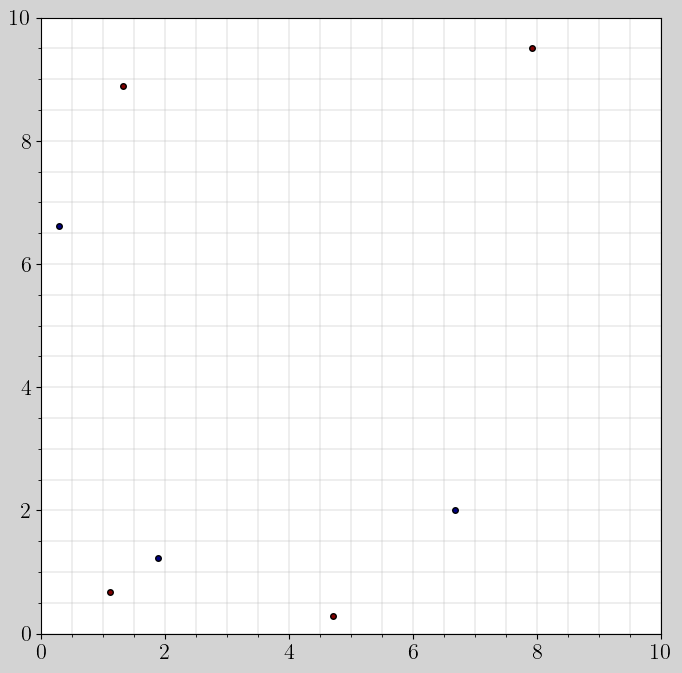
\includegraphics[width=0.4\linewidth]{tarefa-A/posicoes-finais.png}
    \label{fig:posicoes-finais-a}
    \caption{Coordenadas das partículas projetadas à cada $3 \Delta t$.}
\end{figure}

\begin{figure}[h!]
    \centering 
    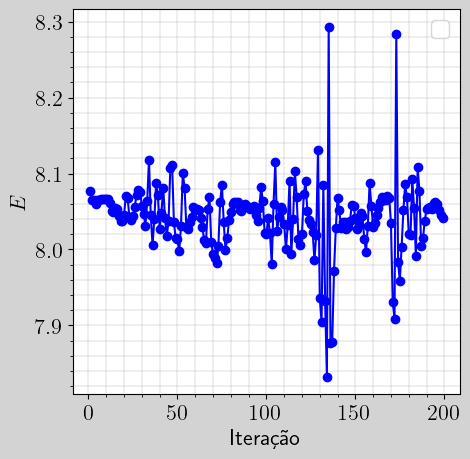
\includegraphics[width=0.4\linewidth]{tarefa-A/energia.png}
    \caption{Energia do sistema à cada $3 \Delta t$.}
    \label{fig:energia_a}
\end{figure}

\clearpage
\subsection*{Código}
O código abaixo está no diretório \verb|tarefa-a/| e contém 
as simulações referentes às tarefas A, B e parte da D.
\begin{minted}{fortran}
    ! Tarefas A, B e parte da D
    implicit real*8(a-h, o-y)
    parameter (pi = acos(-1.e0))
    dimension r_prev(20, 2)
    dimension r_curr(20, 2)
    dimension r_next(20, 2)
    dimension v(20, 2)
    dimension r(20, 20)
    dimension acc(2)
    L = 10
    rL = 10d0
    N = 20

    ! Tarefa A 
    open(unit = 99, file="saidas/tarefa-A/parametros.dat")
    open(unit = 1,  file="saidas/tarefa-A/posicoes-iniciais.dat")
    open(unit = 3,  file="saidas/tarefa-A/evolucao-posicoes.dat")
    ! Tarefa B 
    open(unit = 5,  file="saidas/tarefa-B/velocidades.dat")
    open(unit = 6,  file="saidas/tarefa-B/evolucao-posicoes.dat")
    ! Tarefa D
    open(unit = 9,  file="saidas/tarefa-D/temperatura-b.dat")
    
    dt = 0.02
    v0 = 1.0
    write(99, *) N, L, v0, dt
    close(99)
    ! Defining # rows/columns 
    n_cols = ceiling(sqrt(N*1d0))
    n_rows = ceiling((N*1d0)/(n_cols*1d0)) 
    
    ! Spacing 1/4 
    x_spacing = L/(1d0*n_cols)
    y_spacing = L/(1d0*n_rows)
    spacing = min(x_spacing, y_spacing)/4.0 
    
    ! Centering in the grid
    x_offset = x_spacing / 2.0 
    y_offset = y_spacing / 2.0
    call srand(562369)
    
    k = 1 
    do j = 1, n_rows 
          do i = 1, n_cols 
                r_curr(k, 1) = (i-1)*x_spacing+x_offset
                r_curr(k, 2) = (j-1)*y_spacing+y_offset
                
                r_curr(k, 1) = r_curr(k,1)+(rand())*spacing
                r_curr(k, 2) = r_curr(k,2)+(rand())*spacing
                theta = 2*pi*rand()
                v(k, 1) = v0*cos(theta)
                v(k, 2) = v0*sin(theta)
                
                r_prev(k, 1) = r_curr(k, 1) - v(k, 1) * dt 
                r_prev(k, 2) = r_curr(k, 2) - v(k, 2) * dt 
                k=k+1
          end do 
    end do

    do i = 1, N
          write(1, *) r_curr(i, 1), r_curr(i, 2) 
          write(3, *) 0d0, r_curr(i,1), r_curr(i, 2)
    end do
    close(1)

    DB = 1.0
    ! Dynamics 
    do k = 1, 5000

          t = k * dt 

          acc(1) = 0d0 
          acc(2) = 0d0

          do i = 1, N 
                acc(1) = 0d0 
                acc(2) = 0d0
                do j = 1, N 
                      if(i /= j) then
                           call compute_acc(N,i,j,L,r_curr,acc,r)
                      end if
                end do 
                ! UPDATE POSITIONS
                r_next(i,1) = 2*r_curr(i,1)-r_prev(i,1)+acc(1)*(dt**2)
                r_next(i,2) = 2*r_curr(i,2)-r_prev(i,2)+acc(2)*(dt**2) 

                ! APPLY PBC
                r_next(i,1) = mod(r_next(i,1)+rL, rL)
                r_next(i,2) = mod(r_next(i,2)+rL, rL)

                delta_r_x = delta_pbc(r_next(i,1),r_prev(i,1),L)
                delta_r_y = delta_pbc(r_next(i,2),r_prev(i,2),L)

                ! UPDATE VELOCITIES using adjusted displacements
                v(i, 1) = delta_r_x / (2 * dt)
                v(i, 2) = delta_r_y / (2 * dt)
          end do

          r_prev(:, 1) = r_curr(:, 1)
          r_prev(:, 2) = r_curr(:, 2)
          
          r_curr(:, 1) = r_next(:, 1)
          r_curr(:, 2) = r_next(:, 2)
          
          if(k < 200) then 
                E = 0d0
                call compute_energy(N, L, v, r_curr, E, r)
                write(19,*) k, E
          end if

          ! TAREFA A 
          if(mod(k, 3) == 0 .and. k < 400) then
                do i = 1, N 
                      write(3,*) k, r_curr(i,1),r_curr(i, 2)
                end do
          end if

          ! Tarefa B & D 
          if(mod(k, 20) == 0) then
                do i = 1, N
                      v_mag = sqrt(v(i,1)**2+v(i,2)**2)
                      write(5,*) k, v_mag, v(i,1), v(i,2)
                      write(9,*) .5d0 * v_mag**2
                      write(6,*) k, r_curr(i,1),r_curr(i, 2)
                end do
          end if
    end do
    close(3)
    close(5)
    close(6)
    close(9)
    close(15) 

    end
    ! Submodules for molecular dynamic simulations
    ! Velocity delta 
    function delta_pbc(r_next, r_prev,L)
          implicit real*8(a-h, o-y)
          delta_pbc = r_next - r_prev
          delta_pbc = delta_pbc - L * nint(delta_pbc / L)
    end function delta_pbc

    subroutine initialize_particles(N, L, r_curr,r_prev, v, v0)
          implicit real*8(a-h, o-y)
          dimension r_prev(20, 2)
          dimension r_curr(20, 2)
          dimension v(20, 2)
         
          ! Defining # rows/columns 
          n_cols = ceiling(sqrt(N*1d0))
          n_rows = ceiling((N*1d0)/(n_cols*1d0)) 
          
          ! Spacing 1/4 
          x_spacing = L/(1d0*n_cols)
          y_spacing = L/(1d0*n_rows)
          spacing = min(x_spacing, y_spacing)/4.0 
          
          ! Centering in the grid
          x_offset = x_spacing / 2.0 
          y_offset = y_spacing / 2.0
          call srand(562369)

          k = 1 
          do j = 1, n_rows 
                do i = 1, n_cols 
                      r_curr(k, 1) = (i-1)*x_spacing+x_offset
                      r_curr(k, 2) = (j-1)*y_spacing+y_offset
                      
                      r_curr(k, 1) = r_curr(k,1)+(rand())*spacing
                      r_curr(k, 2) = r_curr(k,2)+(rand())*spacing

                      theta = 2*pi*rand()
                      v(k, 1) = v0*cos(theta)
                      v(k, 2) = v0*sin(theta)
                      
                      r_prev(k, 1) = r_curr(k, 1) - v(k, 1) * dt 
                      r_prev(k, 2) = r_curr(k, 2) - v(k, 2) * dt 
                      k=k+1
                end do 
          end do
    end subroutine initialize_particles

    ! Updates acceleration a = ax, ay 
    ! between particle i and all others
    subroutine compute_acc(N,i,j,L,r_curr,acc, r)
          implicit real*8(a-h, o-y)
          dimension r_curr(20, 2)
          dimension acc(2)
          dimension r(20, 20)
          epsilon = 1e-3

          dx = r_curr(i, 1) - r_curr(j, 1)
          dy = r_curr(i, 2) - r_curr(j, 2)

          dx = dx - L * nint(dx / L)
          dy = dy - L * nint(dy / L)

          r_ij = sqrt(dx**2 + dy**2)
          
          r(i, j) = r_ij 
          r(j, i) = r_ij

          if(r_ij > epsilon .and. r_ij <= 3d0) then 
                F = 24.0 * (2d0/r_ij**13 - 1d0/r_ij**7)
                acc(1) = acc(1) + F * dx / r_ij 
                acc(2) = acc(2) + F * dy / r_ij
          end if 
    end subroutine compute_acc

    subroutine compute_energy(N, L, v, r_curr, E, r)
          implicit real*8(a-h, o-y)
          dimension v(20, 2)
          dimension r_curr(20, 2)
          dimension r(20, 20)
          
          epsilon = 1e-3
          Tk = 0d0
          do i = 1, N
              Tk = Tk + 0.5 * (v(i, 1)**2 + v(i, 2)**2)
          end do
          U = 0d0
          do i = 1, N
            do j = i + 1, N
                r_ij = r(i, j)

                if (r_ij > epsilon .and. r_ij <= 3d0) then
                    U = U + 4 * (r_ij**(-12) - r_ij**(-6))
                end if
            end do
          end do
          E = Tk + U
    end subroutine
\end{minted}
\clearpage
\section{Tarefa B}
\begin{align}
    P(v) &\sim \frac{v^2}{K_B T} \exp \left( - \frac{m v^2}{2K_B T} \right)  \\ 
    P(v_x) &\sim \frac{1}{\sqrt{K_B T}}\exp \left( - \frac{m v_x^2}{2K_B T} \right)\\
    P(v_y) &\sim \frac{1}{\sqrt{K_B T}}\exp \left( - \frac{m v_y^2}{2K_B T} \right)
\end{align}





\begin{figure}[h!]
    \centering
    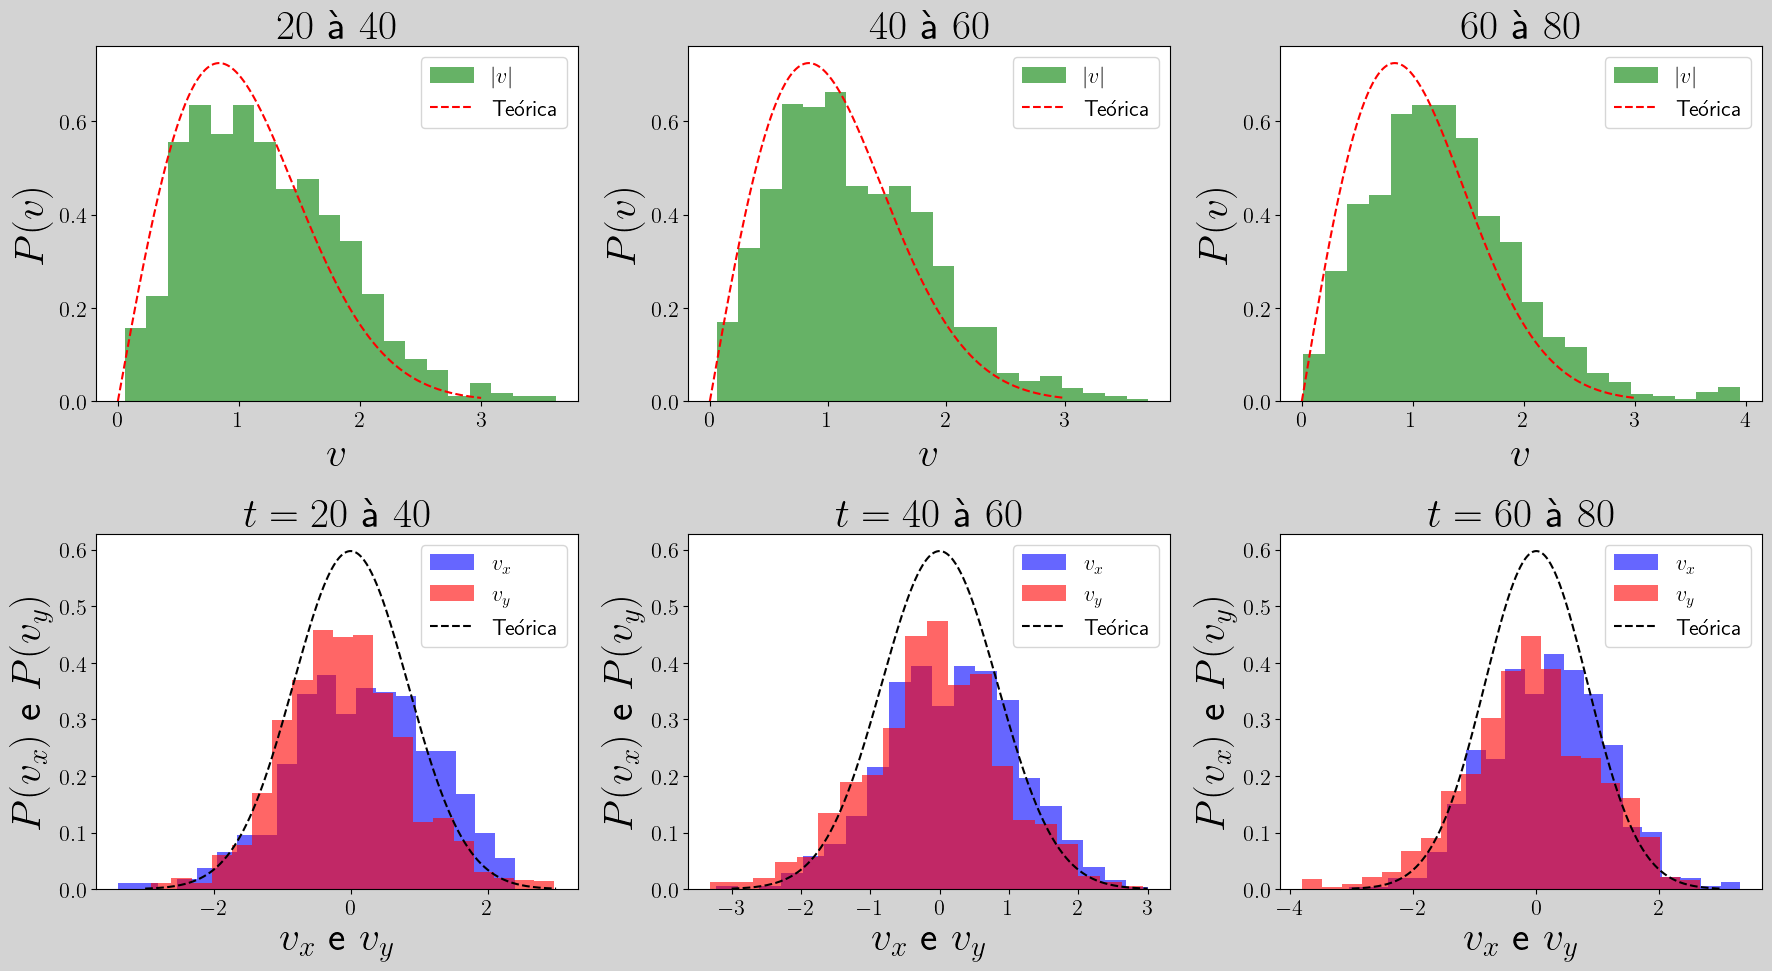
\includegraphics[width=0.7\linewidth]{tarefa-B/distribuicoes-b.png}
    \caption{Distribuição da velocidade, magnitude e componentes em intervalos $t=20-40$, $t=40-60$ e $t=60-80$.}
    \label{fig:distribuicoes-velocidade-b}
\end{figure}


Além disso há um gif para essa simulação.

\clearpage
\section{Tarefa C}
\subsection{C.1 - Histerese }
Segue abaixo a implementação da simulção de histerese:
\begin{minted}{fortran}
            open(1, file="saidas/tarefa-3/saida-tarefa-C1-L60-DB1.dat")
            open(2, file="saidas/tarefa-3/saida-tarefa-C1-L60-DB2.dat")

            open(3, file="saidas/tarefa-3/saida-tarefa-C1-L80-DB1.dat")
            open(4, file="saidas/tarefa-3/saida-tarefa-C1-L80-DB2.dat")

            open(5, file="saidas/tarefa-3/saida-tarefa-C1-L100-DB1.dat")
            open(6, file="saidas/tarefa-3/saida-tarefa-C1-L100-DB2.dat")


            call tarefaC1(60, 0.001, 1)
            call tarefaC1(60, 0.0001,  2)

            call tarefaC1(80, 0.001, 3)
            call tarefaC1(80, 0.0001, 4)

            call tarefaC1(100,0.001, 5)
            call tarefaC1(100,0.0001, 6)

            do i = 1, 6
                close(i)
            end do
            end

            subroutine tarefaC1(L_real, dbeta, f_name)
                implicit integer(f-f)
            !           Tarefa B - Recozimento e quenching
                implicit real(j-j, m-m)
                parameter(L = 100)
                dimension exps(-4:4)
                byte lattice(1:L, 1:L)

                ! periodic boundary conditions
                dimension ipbc(0:L+1)

                do i = 1, L_real
                    ipbc(i) = i
                end do  

                ipbc(0) = L_real
                ipbc(L_real+1) = 1

                N = L_real * L_real

                mag = 0.0d0

                call srand(96312)
                ! b = 0
                call initialize_random_lattice(lattice,  L_real, L_real)

                call total_magnetization(lattice, mag, L_real)

                ! initial energy
                E = H_0(lattice, ipbc, L_real)

                beta = 0.0

                write(f_name, *) 0, beta,  mag, E/N

                imax = int(1.75 / dbeta) + 1 

                do i = 1, imax

                    call define_exponentials(exps, beta)

                    if(i < imax/ 2) then 
                        beta = beta + dbeta 
                    else
                        beta = beta - dbeta 
                    end if  

                    do k = 1 , N
                        call flip_spin(lattice,ipbc,exps,E,mag,L_real)
                    end do   

                    write(f_name, *) i, beta, mag, E/N

                end do
            end subroutine tarefaC1
\end{minted}


No gráfico (\ref{fig:c1_dbeta1}) temos o comportamento da energia média por spin na dinâmica do loop
térmico e o gráfico de histerese, isto é, a energia média em relação à $\beta$ para 
variações de $\Delta b = 0,001$. 

\begin{figure}
    \centering
    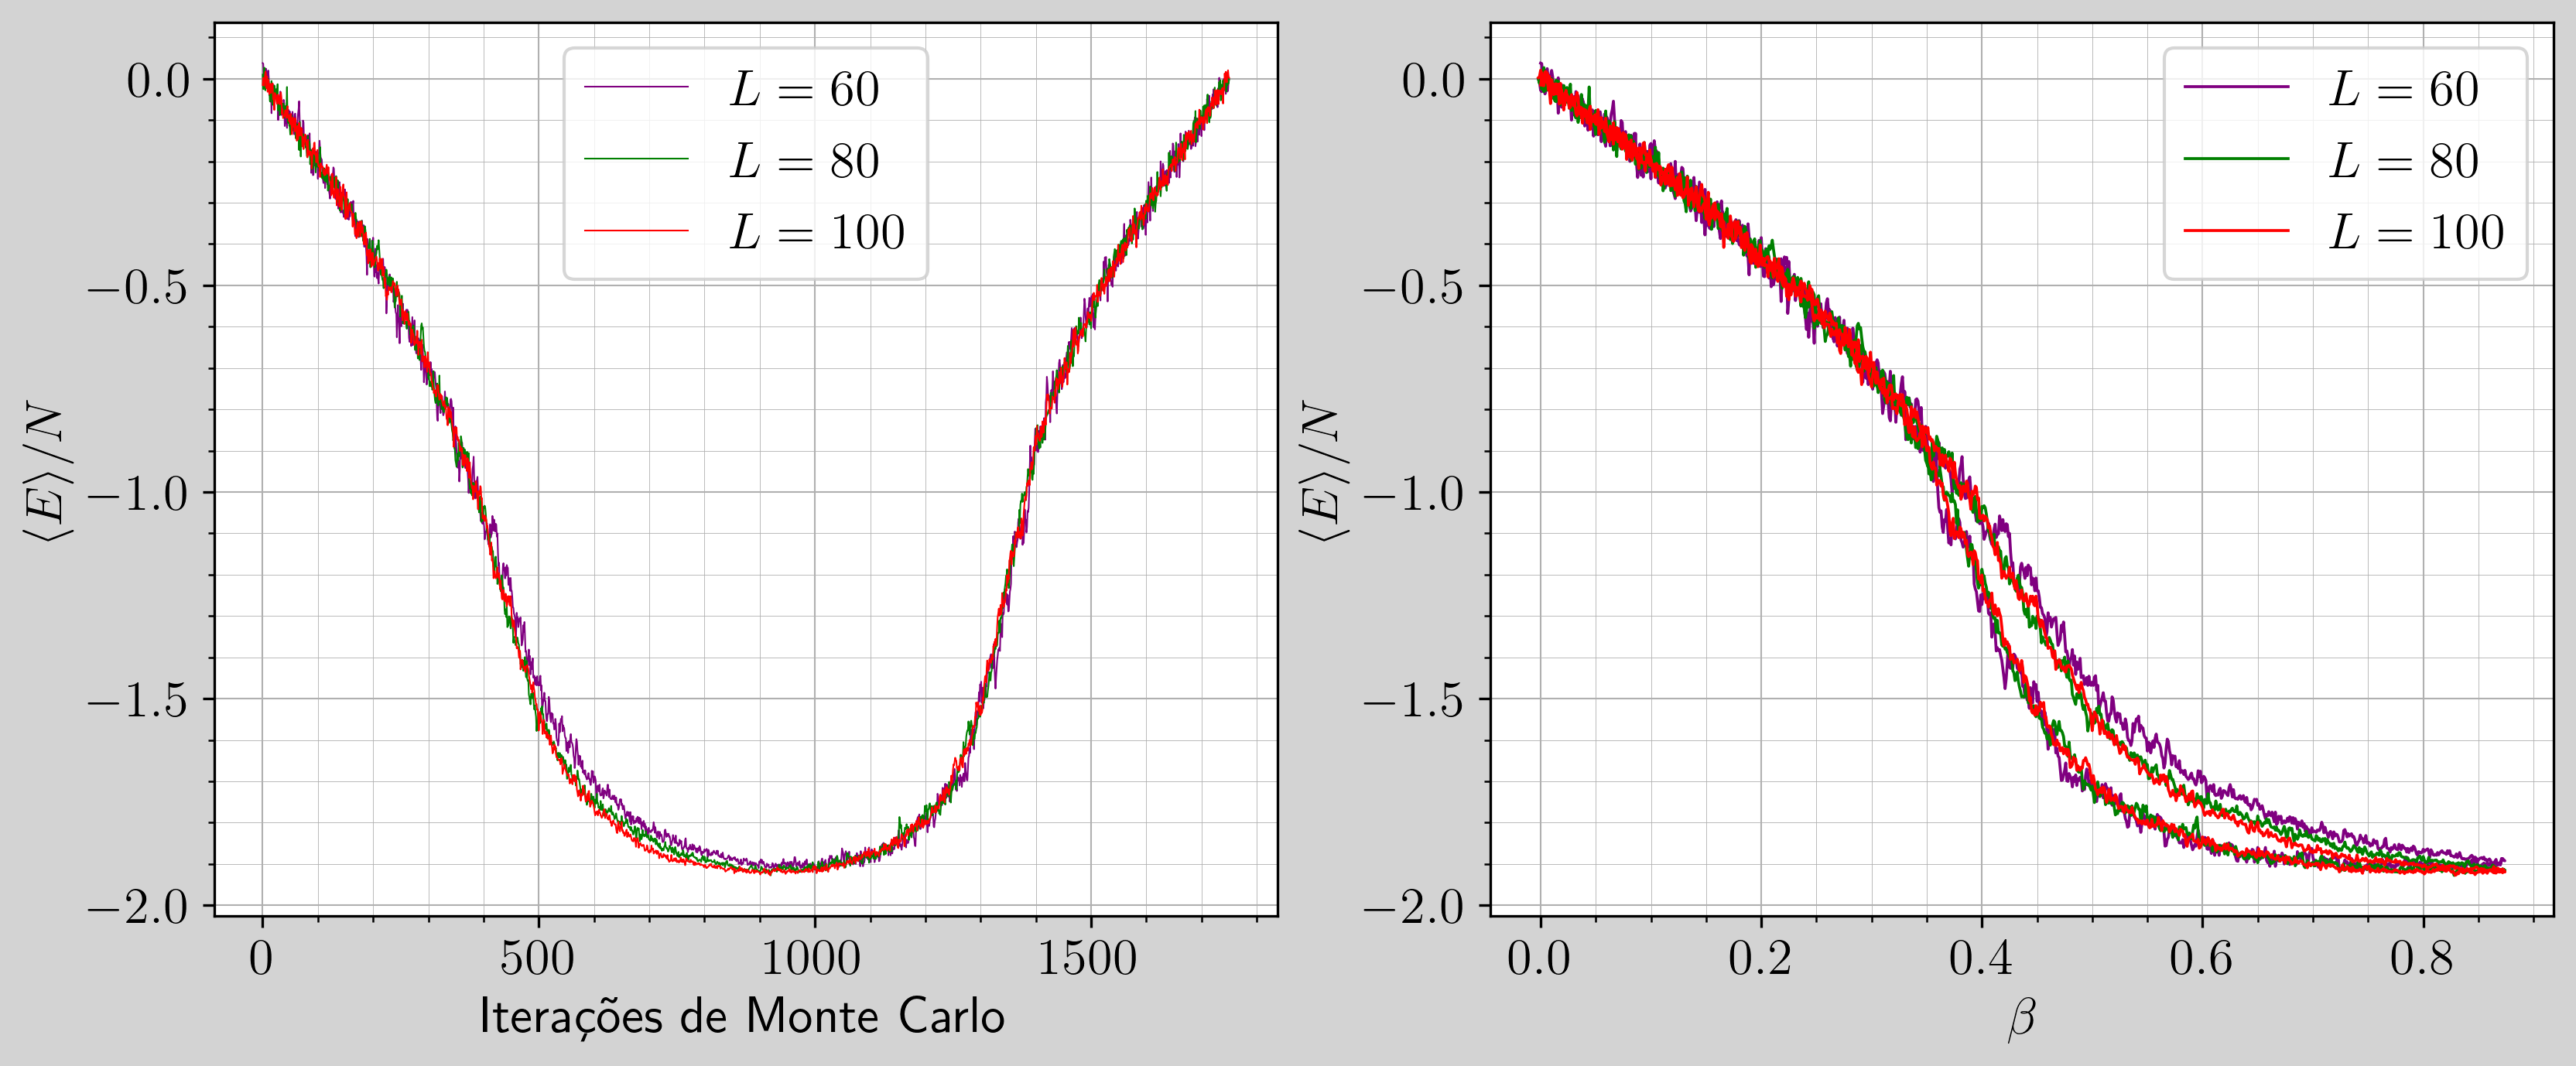
\includegraphics[width=0.8\linewidth]{graficos/tarefa-3/graf-tarefa-C1-delta1.png}
    \caption{À esquerda energia média por spin por iterações de Monte Carlo e à direita em relação à $\beta$.}
    \label{fig:c1_dbeta1}
\end{figure}


A figura (\ref{fig:c1_dbeta2}) equivale a dinâmica como a anterior, mas com uma variação 
$\Delta \beta = 0,0001$, que fornece um resultado com menos flutuações, sobretudo para as redes maiores.

\begin{figure}
    \centering
    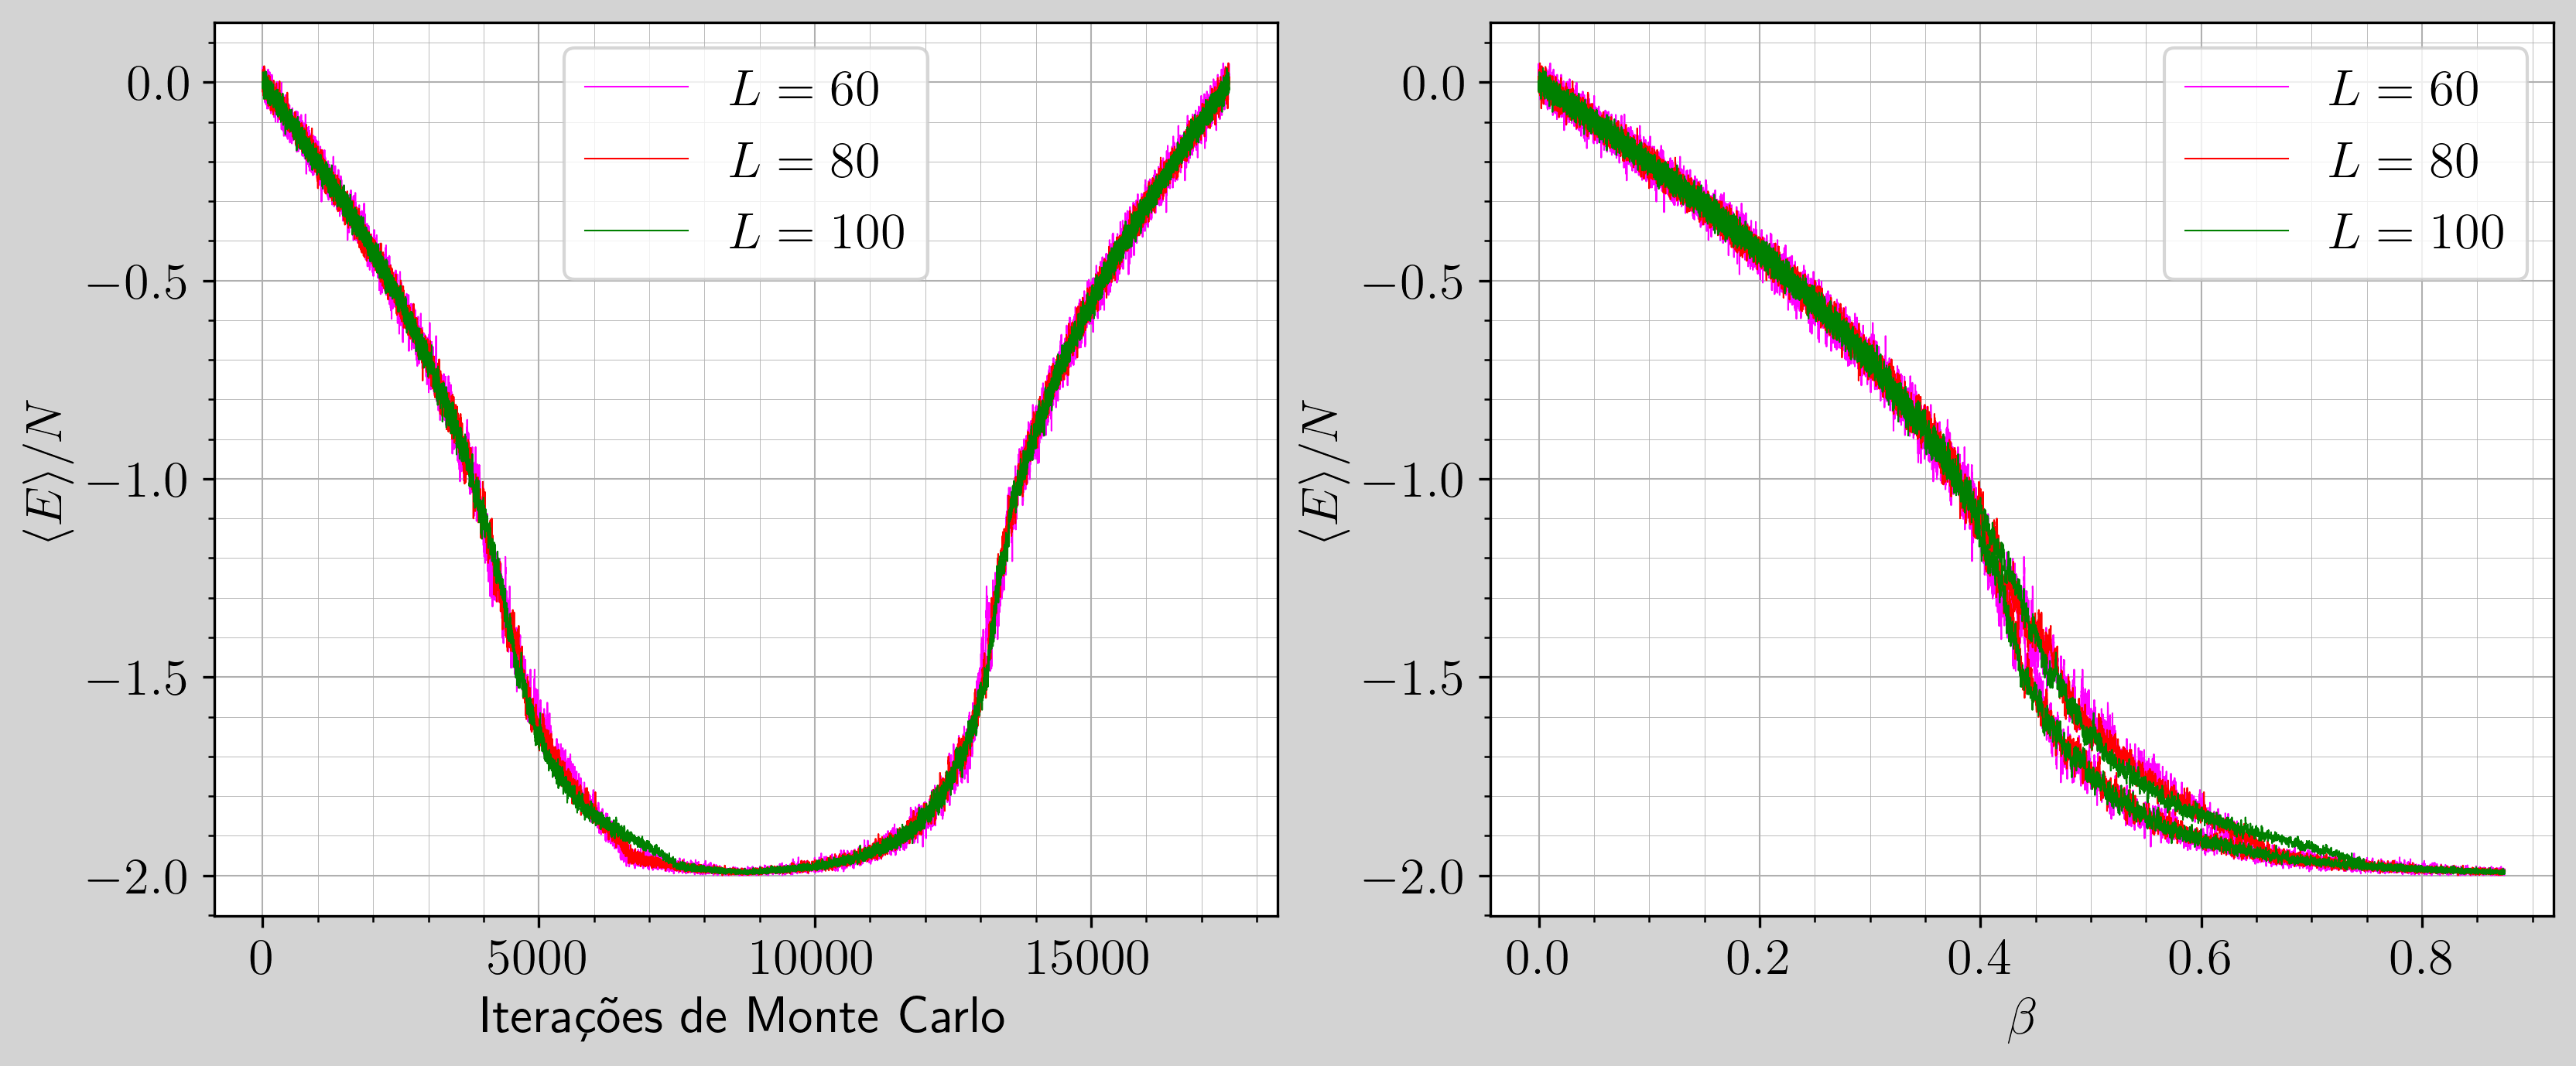
\includegraphics[width=0.8\linewidth]{graficos/tarefa-3/graf-tarefa-C1-delta2.png}
    \caption{À esquerda energia média por spin por iterações de Monte Carlo e à direita em relação à $\beta$.}
    \label{fig:c1_dbeta2}
\end{figure}

Podemos observar nos gráficos que a região de histerese correspondem à um intervalo de $\beta$ entre $0,4$ e 
$0,6$, mas apenas a partir dessas medidas não conseguimos ter uma boa precisão dessa medida.

\subsection{C.2 - Temperatura crítica }


\begin{marginfigure}
    \centering
    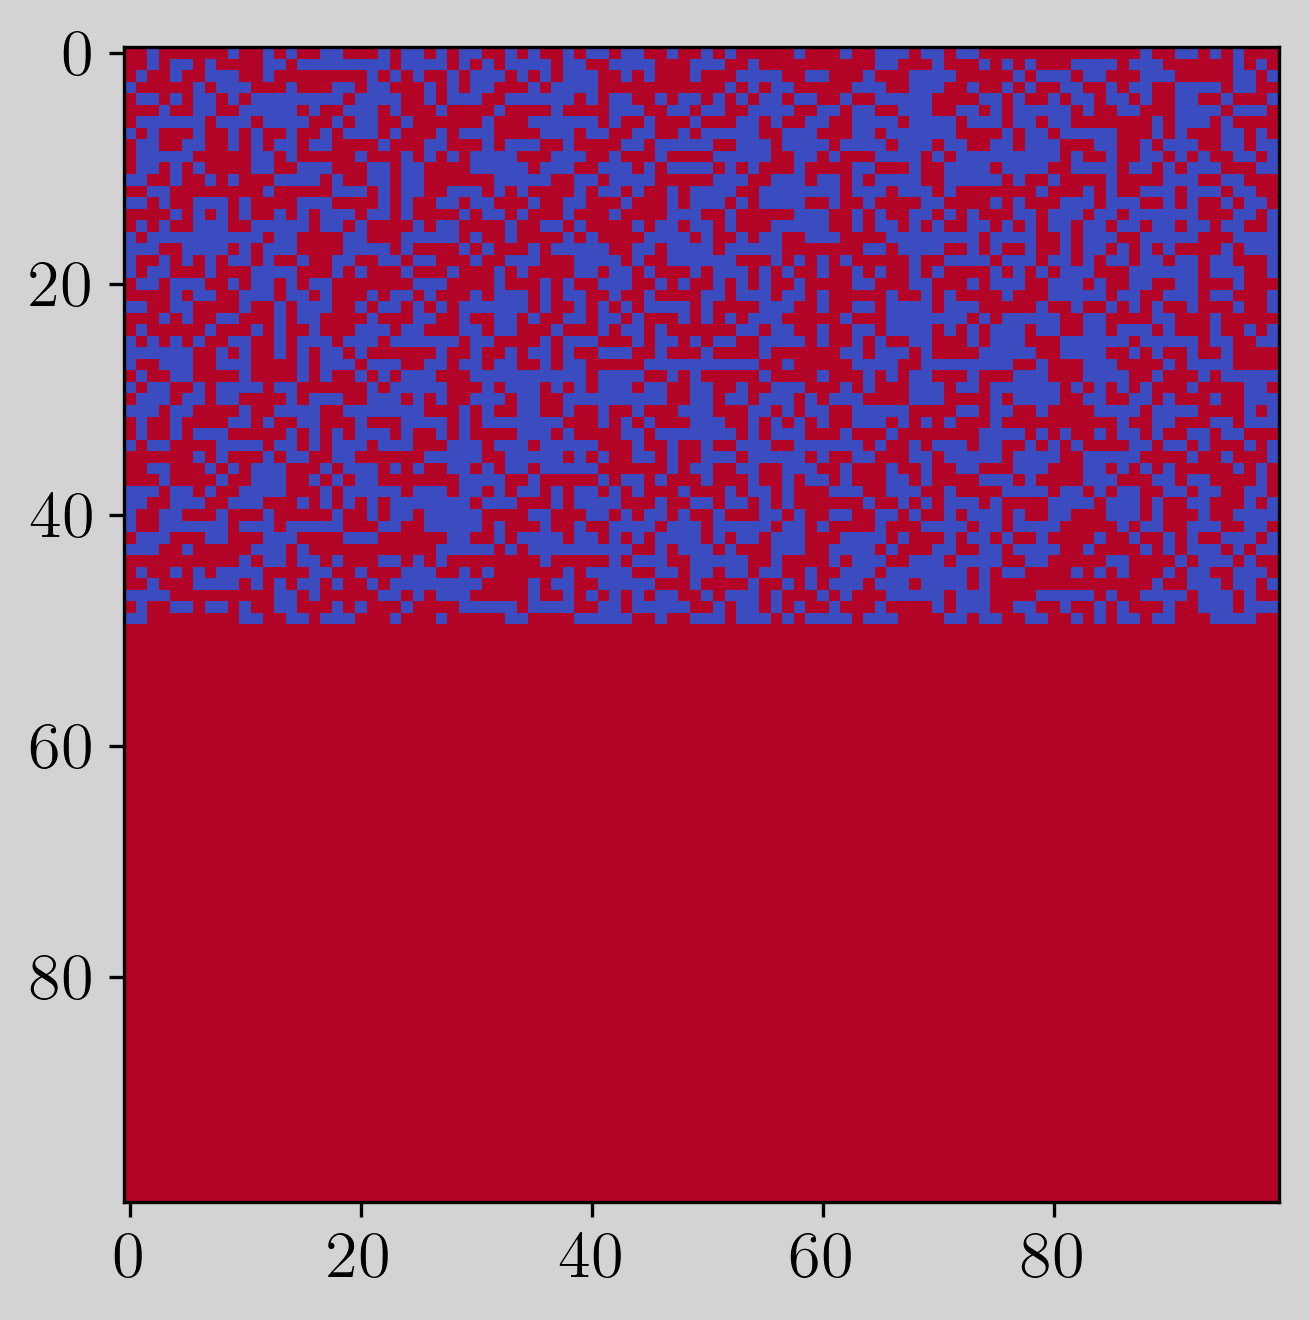
\includegraphics[width=\linewidth]{graficos/tarefa-3/graf-tarefa-C2-conf.png}
    \caption{Configuração inicial para dinâmica utilizada na medida de temperatura crítica.}
    \label{fig:c2_conf_inicial}
\end{marginfigure}


Modificação no código do item anterior: 

\begin{minted}{fortran}

        dimension betas(1:5)
        parameter(betas = (/0.41, 0.44, 0.47, 0.51, 0.55/))

        open(1, file="saidas/tarefa-3/saida-tarefa-C2-L60-b1.dat")
        open(2, file="saidas/tarefa-3/saida-tarefa-C2-L60-b2.dat")
        open(3, file="saidas/tarefa-3/saida-tarefa-C2-L60-b3.dat")
        open(4, file="saidas/tarefa-3/saida-tarefa-C2-L60-b4.dat")
        open(5, file="saidas/tarefa-3/saida-tarefa-C2-L60-b5.dat")

        do i = 1, 5
            call tarefaC2(60, betas(i), i)
            close(1)
        end do

        open(1, file="saidas/tarefa-3/saida-tarefa-C2-L80-b1.dat")
        open(2, file="saidas/tarefa-3/saida-tarefa-C2-L80-b2.dat")
        open(3, file="saidas/tarefa-3/saida-tarefa-C2-L80-b3.dat")
        open(4, file="saidas/tarefa-3/saida-tarefa-C2-L80-b4.dat")
        open(5, file="saidas/tarefa-3/saida-tarefa-C2-L80-b5.dat")

        do i = 1, 5
            call tarefaC2(80, betas(i), i)
            close(1)
        end do

        open(1, file="saidas/tarefa-3/saida-tarefa-C2-L100-b1.dat")
        open(2, file="saidas/tarefa-3/saida-tarefa-C2-L100-b2.dat")
        open(3, file="saidas/tarefa-3/saida-tarefa-C2-L100-b3.dat")
        open(4, file="saidas/tarefa-3/saida-tarefa-C2-L100-b4.dat")
        open(5, file="saidas/tarefa-3/saida-tarefa-C2-L100-b5.dat")

        do i = 1, 5
            call tarefaC2(100, betas(i), i)
            close(1)
        end do
        end
        subroutine tarefaC2(L_real, beta, fname)
!               Tarefa B - Recozimento e quenching
            implicit integer(f-f)
            implicit real(j-j, m-m)
            parameter(L = 100)
            dimension exps(-4:4)
            byte lattice(1:L, 1:L)
            ! periodic boundary conditions
            dimension ipbc(0:L+1)

            do i = 1, L_real
                ipbc(i) = i
            end do  

            ipbc(0) = L_real
            ipbc(L_real+1) = 1

            N = L_real * L_real

            mag = 0.0d0

            call srand(L_real * 392)

            ! half ordered / half random.
            call initialize_lattice(lattice, L_real, L_real)
            call initialize_random_lattice(lattice,  L_real/2, L_real)

            open(99, file = "saidas/tarefa-3/saida-tarefa-C2-conf.dat")
            call write_lattice(lattice, L_real, 99)
            close(99)

            call total_magnetization(lattice, mag, L_real)

            ! initial energy
            E = H_0(lattice, ipbc, L_real)
            dbeta = 0.01
            write(fname, *) 0, E/N
            do i = 1, 3000
                call define_exponentials(exps, beta)
                do k = 1 , N
                    call flip_spin(lattice,ipbc,exps,E,mag,L_real)
                end do   
                write(fname, *) i, E/N
            end do
        end subroutine tarefaC2
\end{minted}


\begin{marginfigure}
    \centering
    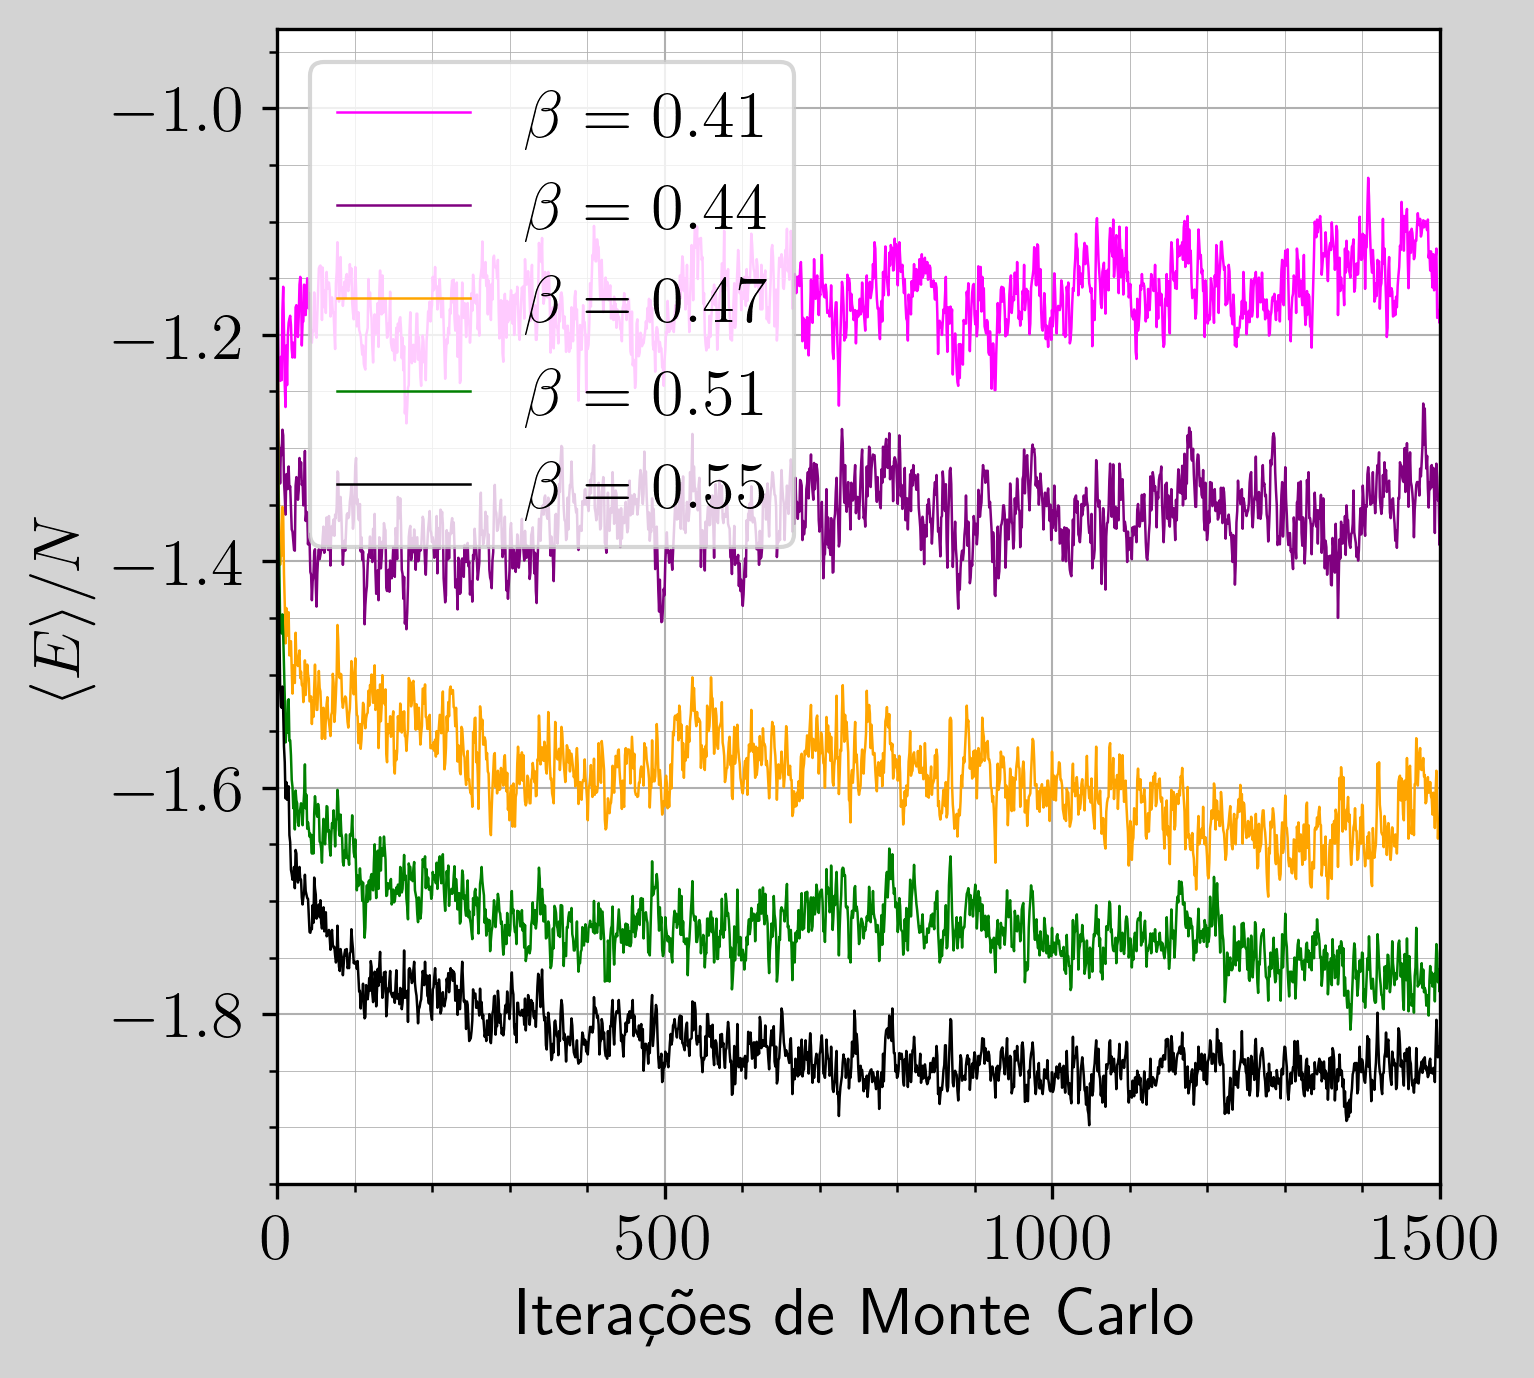
\includegraphics[width=\linewidth]{graficos/tarefa-3/graf-tarefa-C2-L80.png}
    \caption{Dinâmica para L=80.}
    \label{fig:c2_l80}
\end{marginfigure}

Partimos dos resultados do item anterior e tentamos obter a temperatura crítica do modelo. Para isso observamos
a variação de energia no intervalo $\beta$ discutido antes, isto é, $0,4 < \beta < 0.6$. 
A imagem (\ref{fig:c2_conf_inicial}) mostra a configuração inicial do sistema. Foram escolhidos alguns 
valores de $\beta$ para executar a dinâmica de Monte Carlo. 


\begin{marginfigure}
    \centering
    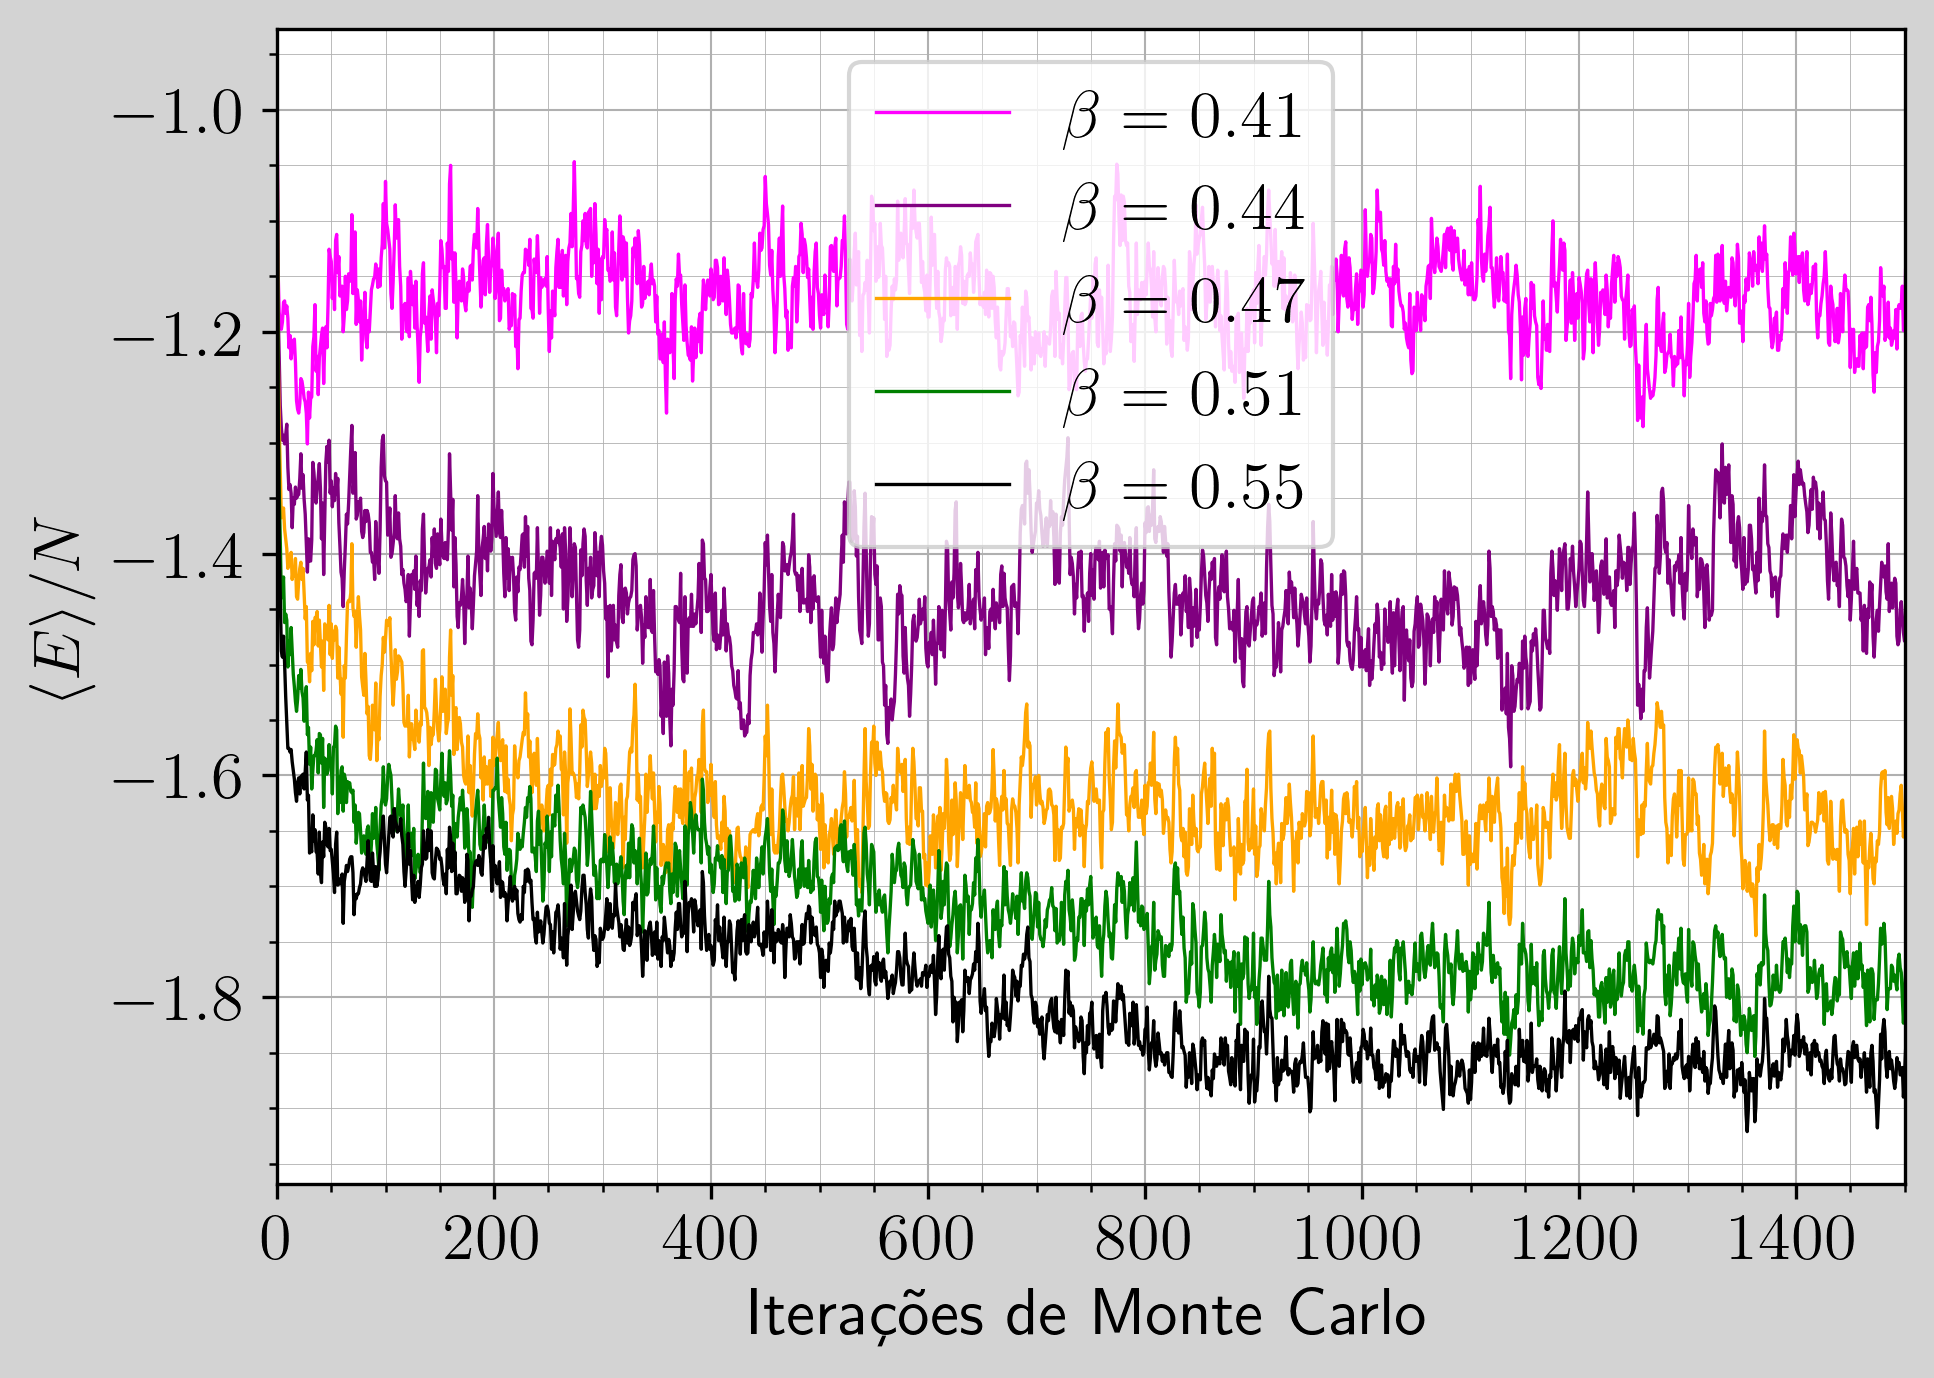
\includegraphics[width=\linewidth]{graficos/tarefa-3/graf-tarefa-C2-L60.png}
    \caption{Dinâmica para L=60.}
    \label{fig:c2_l60}
\end{marginfigure}



Nas figuras (\ref{fig:c2_l60}), (\ref{fig:c2_l80}) e (\ref{fig:c2_l100}) estão 
as evoluções, em um intervalo de passos de Monte Carlo reduzido, da energia média por spin. 

\clearpage
Nota-se que as energias médias por spin sempre partem do mesmo valor no intervalo da histerese e a 
que possui maior variação é a que corresponde à $\beta = 0.44$, esse é o $\beta$ relacionado à temperatura crítica $T_c = 1/\beta_c \approx 2,27$ .

\begin{figure}
    \centering
    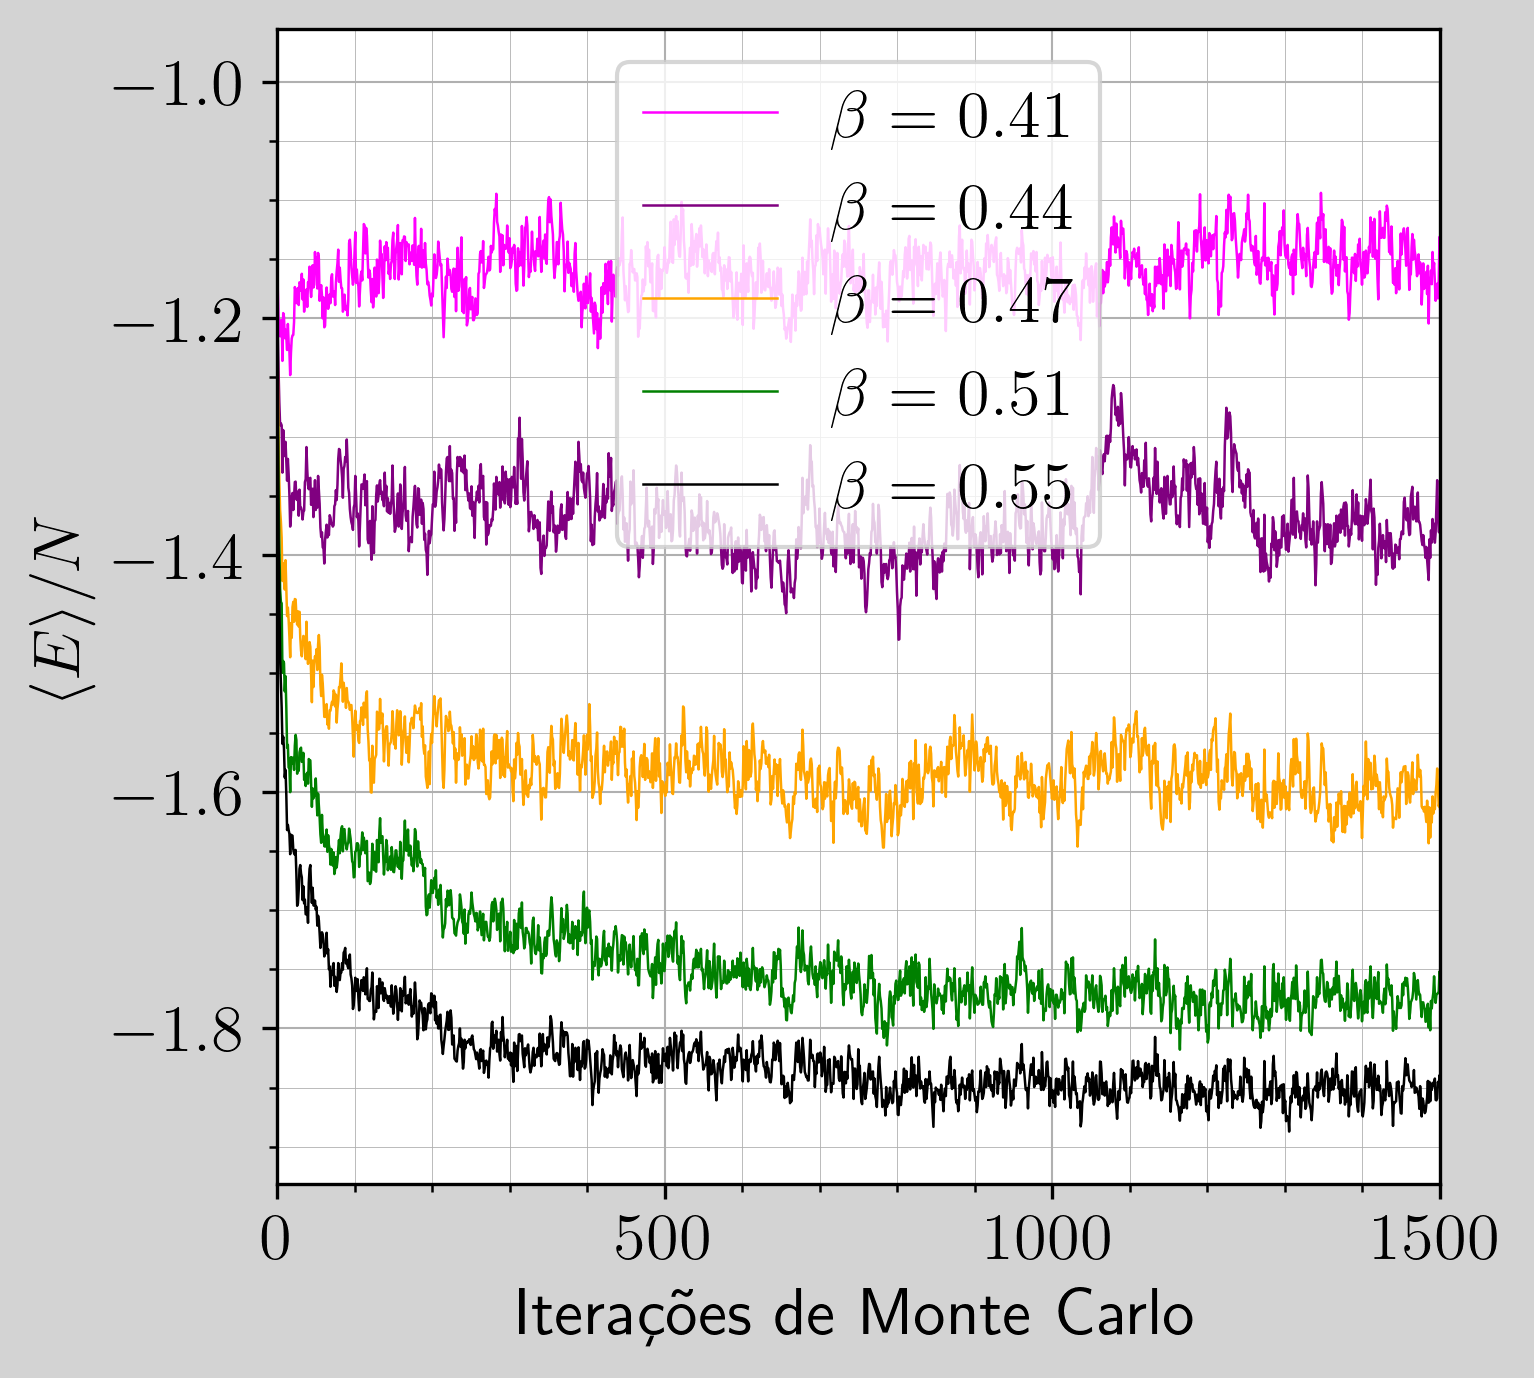
\includegraphics[width=0.5\linewidth]{graficos/tarefa-3/graf-tarefa-C2-L100.png}
    \caption{Dinâmica para L=100.}
    \label{fig:c2_l100}
\end{figure}

Além disso, pela (\ref{eq:calor_especifico}) podemos constatar que esse $\beta_c = 0,44$ também está associado à 
um valor específico crítico no modelo. 
\section{Tarefa D}
Nessa tarefa o nosso interesse é estudar o fenômeno de quebra espontânea de simetria. 
Queremos mostrar que o tempo que um sistema leva para mudar toda a orientação de magnetização cresce de forma 
exponencial com a dimensão da malha utilizada. 
Para isso foi implementado uma simulação que executa passos de Monte Carlo e contabiliza o intervalo 
de tempo de Monte Carlo que o sistema leva para mudar a magnetização conforme o tamanho $L$ da rede aumenta. 

O código em fortran para essa simulação está abaixo: 

\begin{minted}{fortran}
    implicit integer(f-f)
    implicit real(m-m)
    parameter(L = 100)
    dimension exps(-4:4)
    byte lattice(1:L, 1:L)
    ! periodic boundary conditions
    dimension ipbc(0:L+1)
    ! this or using mod
    open(unit=1, file="saidas/tarefa-4/saida-tarefa-D.dat")
    open(unit=2, file="saidas/tarefa-4/saida-tarefa-MAG_T.dat")
    beta = 0.5
    call define_exponentials(exps, beta)
    do L_real = 4, 10
        print *, "L = ", L_real 
        call srand(3519) ! /L_real+1)
        N = L_real * L_real
        ! setting ipbc
        do i = 1, L_real
            ipbc(i) = i
        end do  
        ipbc(0) = L_real
        ipbc(L_real+1) = 1
        mag = 0.0e0
        call initialize_random_lattice(lattice, L_real, L_real)
        call total_magnetization(lattice, mag, L_real)
        n_inversions = 10000
        n_curr = 0
        n_time = 0
        do while(n_curr < n_inversions) 
            mag_prev = mag
            do i = 1, N
                call flip_spin(lattice, ipbc, exps, E, mag, L_real)
            end do
            n_time = n_time + 1
            ! Fazer o gráfico da magnetização aqui.
            if(mag_prev * mag < 0) then 
                t_mean = t_mean + n_time
                n_time = 0
                n_curr = n_curr + 1
            end if
        end do
        write(2, *) t_mean, mag
        t_mean = t_mean / n_inversions
        write(1, *) L_real, t_mean
    end do
    close(1)
    end
\end{minted}

Podemos ver pela figura(\ref{fig:d_graficos}) que o intervalo cresce de forma exponencial com 
o tamanho $L$ da malha: 

\begin{figure}
    \centering
    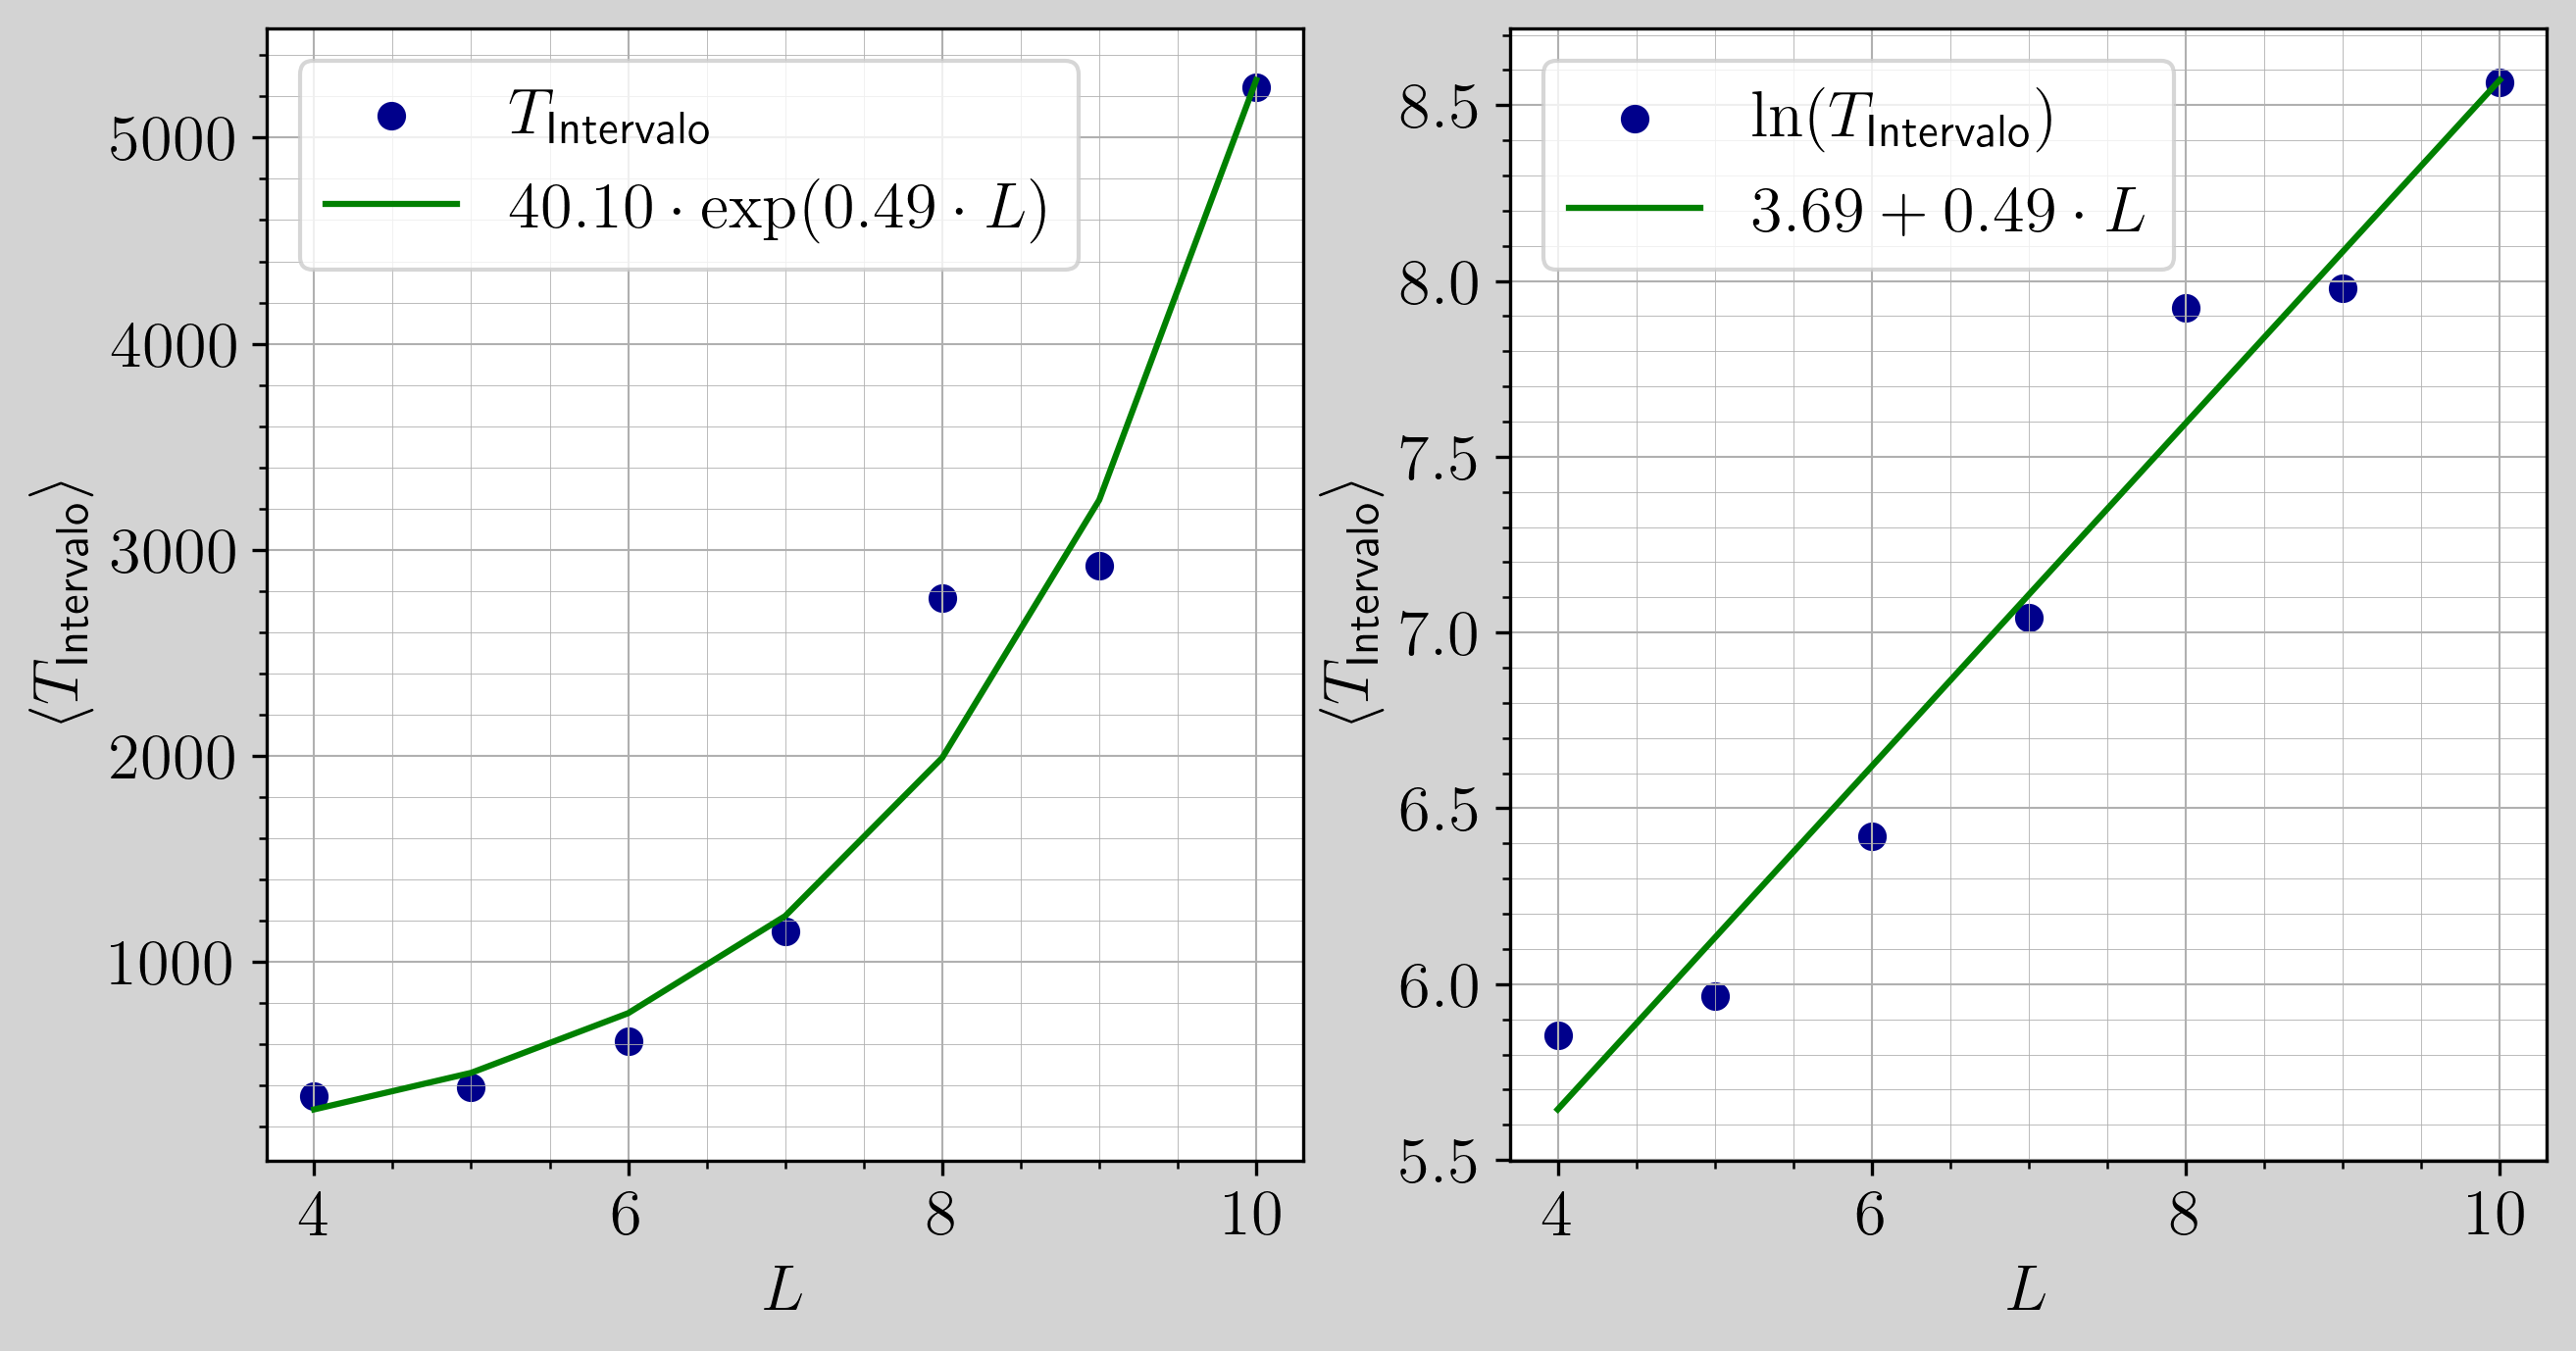
\includegraphics[width=\linewidth]{graficos/tarefa-4/graf-tarefa-D.png}
    \caption{Gráfico do crescimento do intervalo $\langle T_\text{intervalo} \rangle$ em função de $L$ e ajuste linear.}
    \label{fig:d_graficos}
\end{figure}

Para implementação com número de inversões da ordem de $10^4$ foi obtido o ajuste linear 
$\ln\left(\langle T_{\text{intervalo}}(L)\rangle\right)  \approx 3,67 + 0,49 \cdot L$. 

Essa dependência exponencial para que ocorra quebra da simetria talvez explique o que ocorre na simulação da tarefa B
em que o sistema atinge o equilibrio mas a magnetização tem comportamento não usual. Aumentando o número de passos 
de Monte Carlo naquela simulação pode resolver o aparente problema.
\section{Tarefa E}
Agora que estudamos a dinâmica molecular e conseguimos atingir observar o que as velocidades 
seguem distribuições de Maxwell-Boltzman, queremos impor uma dinâmica específica sobre o 
gás 2D. 
Nesse caso queremos observar a cristalização de moleculas, e para isso consideramos uma caixa 
de tamanho $L=4$ com $N = 16$ partículas, ou seja, a densidade nesse caso é $\sigma = 1$, o passo 
foi $\Delta t = 0.005$ e a velocidade inicial de teste $v_0 = 1$. 
No entanto, para essa velocidade não foi possível observar a cristalização acontecendo nos diferentes regimes
de temo desejados, por isso foi necessário diminuir a velocidade inicial $v_0$ para 
$v_0 = 0.2$. Isso condiz com um sistema à baixa temperaturas de alta densidade. 

Como pode ver abaixo (\ref{fig:posicoes-finais-e}) correspondem à cristalização das moléculas. 
Da esquerda para a direita temos o ``rastro'' das partículas nos temos $0 \leq t \leq 0.1$, $0.2 \leq t \leq 0.4$ e 
por fim $13 \leq t \leq 16$. Foram consideradas as posições em intervalos de $ 10 \Delta t$. 

\begin{figure}[h!]
    \centering
    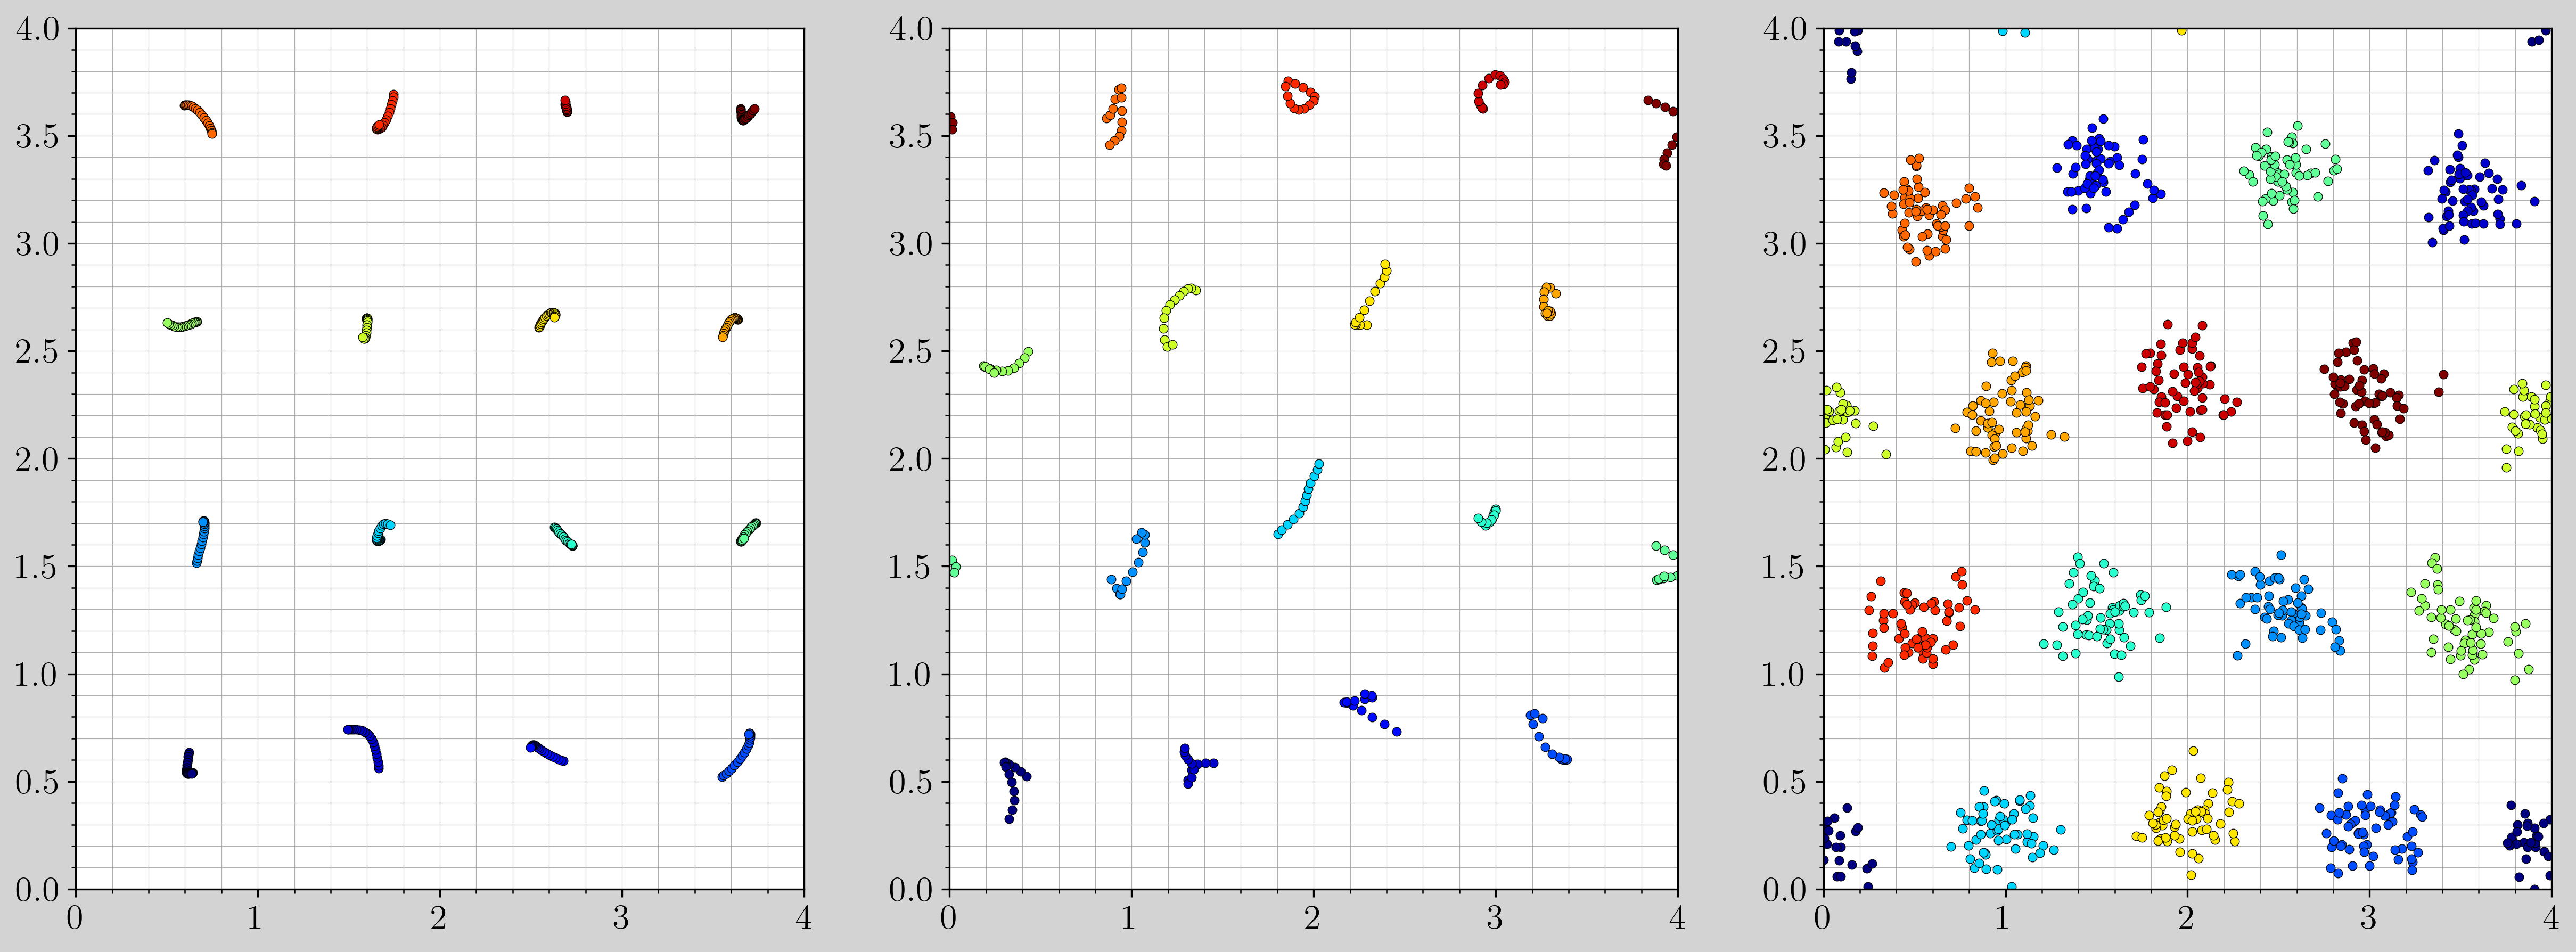
\includegraphics[width=0.95\linewidth]{tarefa-E/posicoes-finais.png}
    \caption{Etapas da cristalização das moléculas.}
    \label{fig:posicoes-finais-e}
\end{figure}


Além desse gráfico foi construido um vídeo para essa tarefa. Esse é um pouco mais longo que os anteriores\footnote{E espero que consiga subir ele para o basalto.}
mas observando apenas os segundos finais dele podemos notar que as partículas permanecem quase presas em uma determinada região nas proximidades da 
do ponto de cristalização. É possível até perceber a estrutura triangular com a qual as partículas se movimentam em torno dos vizinhos. 

\subsection*{Implementação - Simulação E}
\begin{minted}{fortran}

      ! TAREFA E 
      implicit real*8(a-h, o-y)
      parameter (pi = acos(-1.e0))
      dimension r_prev(20, 2)
      dimension r_curr(20, 2)
      dimension r_next(20, 2)
      dimension v(20, 2)
      dimension acc(2)
      dimension r(20, 20)

      open(unit=75, file="saidas/tarefa-E/parametros.dat")
      open(unit=76, file="saidas/tarefa-E/posicoes-iniciais.dat")
      open(unit=77, file="saidas/tarefa-E/evolucao-posicoes-1.dat")
      open(unit=78, file="saidas/tarefa-E/evolucao-posicoes-2.dat")
      open(unit=79, file="saidas/tarefa-E/evolucao-posicoes-3.dat")

      ! Reset variables: 
      r_prev = 0
      r_curr = 0
      r_next = 0
      v = 0

      L = 4
      rL = 4d0
      N = 16
      dt = 5e-3

      v0 = 0.2

      write(75, *) N, L, v0, dt 
      close(75)

      ! Initialize particles 

      n_cols = ceiling(sqrt(N*1d0))
      n_rows = ceiling((N*1d0)/(n_cols*1d0)) 
      
      ! Spacing 1/4 
      x_spacing = L/(1d0*n_cols)
      y_spacing = L/(1d0*n_rows)
      spacing = min(x_spacing, y_spacing)/4.0 
      
      ! Centering in the grid
      x_offset = x_spacing / 2.0 
      y_offset = y_spacing / 2.0
      
      call srand(3512341)

      k = 1 
      do j = 1, n_rows 
            do i = 1, n_cols 
                  r_curr(k, 1) = (i-1)*x_spacing+x_offset
                  r_curr(k, 2) = (j-1)*y_spacing+y_offset
                  
                  r_curr(k, 1) = r_curr(k,1)+(rand())*spacing
                  r_curr(k, 2) = r_curr(k,2)+(rand())*spacing
                  
                  theta = 2*pi*rand()
                  
                  v(k, 1) = v0*cos(theta)
                  v(k, 2) = v0*sin(theta)
                  
                  r_prev(k, 1) = r_curr(k, 1) - v(k, 1) * dt 
                  r_prev(k, 2) = r_curr(k, 2) - v(k, 2) * dt 
                  k=k+1
            end do 
      end do

      do i = 1, N 
            write(76, *) r_curr(i, 1), r_curr(i, 2)
      end do 
      close(76)

      ! Dynamics 
      do k = 1, 3200 
            t = k * dt 
            acc(1) = 0d0 
            acc(2) = 0d0
            do i = 1, N 
                  acc(1) = 0d0 
                  acc(2) = 0d0
                  do j = 1, N 
                        if(i /= j) then
                        call compute_acc(N,i,j,L,r_curr,acc, r)
                        end if
                  end do 
                  ! UPDATE POSITIONS
                  r_next(i,1) = 2*r_curr(i,1)-r_prev(i,1)+acc(1)*(dt**2)
                  r_next(i,2) = 2*r_curr(i,2)-r_prev(i,2)+acc(2)*(dt**2) 

                  ! APPLY PBC
                  r_next(i,1) = mod(r_next(i,1)+rL, rL)
                  r_next(i,2) = mod(r_next(i,2)+rL, rL)

                  delta_r_x = delta_pbc(r_next(i,1),r_prev(i,1),L)
                  delta_r_y = delta_pbc(r_next(i,2),r_prev(i,2),L)

                  ! UPDATE VELOCITIES using adjusted displacements
                  v(i, 1) = delta_r_x / (2 * dt)
                  v(i, 2) = delta_r_y / (2 * dt)
            end do
            r_prev(:, 1) = r_curr(:, 1)
            r_prev(:, 2) = r_curr(:, 2)
            
            r_curr(:, 1) = r_next(:, 1)
            r_curr(:, 2) = r_next(:, 2)

            if(k < 21) then 
                  do i = 1, N 
                        write(77,*) k, r_curr(i,1),r_curr(i,2)
                  end do
            else if (k > 40 .and. k < 81 .and. mod(k,3)==0) then 
                  do i = 1, N 
                        write(78,*) k, r_curr(i,1),r_curr(i,2)
                  end do
            else if (k > 2600 .and. k < 3200 .and. mod(k,10)==0) then 
                  do i = 1, N 
                        write(79,*) k, r_curr(i,1),r_curr(i,2)
                  end do
            end if 
      end do 
      close(77)
      close(78)
      close(79)
      end
      function delta_pbc(r_next, r_prev,L)
            implicit real*8(a-h, o-y)
            delta_pbc = r_next - r_prev
            delta_pbc = delta_pbc - L * nint(delta_pbc / L)
      end function delta_pbc
      ! Updates acceleration a = ax, ay 
      ! between particle i and all others
      subroutine compute_acc(N,i,j,L,r_curr,acc, r)
            implicit real*8(a-h, o-y)
            dimension r_curr(20, 2)
            dimension acc(2)
            dimension r(20, 20)
            epsilon = 1e-3

            dx = r_curr(i, 1) - r_curr(j, 1)
            dy = r_curr(i, 2) - r_curr(j, 2)

            dx = dx - L * nint(dx / L)
            dy = dy - L * nint(dy / L)

            r_ij = sqrt(dx**2 + dy**2)
            
            r(i, j) = r_ij 
            r(j, i) = r_ij

            if(r_ij > epsilon .and. r_ij <= 3d0) then 
                  F = 24.0 * (2d0/r_ij**13 - 1d0/r_ij**7)
                  acc(1) = acc(1) + F * dx / r_ij 
                  acc(2) = acc(2) + F * dy / r_ij
            end if 
      end subroutine compute_acc

      subroutine compute_energy(N, L, v, r_curr, E, r)
            implicit real*8(a-h, o-y)
            dimension v(20, 2)
            dimension r_curr(20, 2)
            dimension r(20, 20)
            
            epsilon = 1e-3
            Tk = 0d0
            do i = 1, N
                Tk = Tk + 0.5 * (v(i, 1)**2 + v(i, 2)**2)
            end do
            U = 0d0
            do i = 1, N
              do j = i + 1, N
                  r_ij = r(i, j)

                  if (r_ij > epsilon .and. r_ij <= 3d0) then
                      U = U + 4 * (r_ij**(-12) - r_ij**(-6))
                  end if
              end do
            end do
            E = Tk + U
      end subroutine
\end{minted}
\clearpage 
\section{Tarefa F}
Por fim, queremos elaborar um pouco mais a dinâmica da tópico anterior(\ref{sec:secE}). 
Agora iremos impor uma fusão à um sólido. Para isso consideraremos um sistema de mesmas dimensões que o anterior 
e executaremos a dinâmica normalmente até atingir a cristalização como antes. A partir desse ponto
nosso impomos uma dinâmica externa às moléculas aumentando sua velocidade por um fator $\gamma = 1.5$. Repetimos 
essa dinâmica até que o sistema atinja um novo equilíbrio térmico. 

A imposição de novas velocidades é dada por 

\begin{equation}
    \mathbf{r}_{\text{anterior}} \longleftarrow \mathbf{r}_{\text{atual}} - (\mathbf{r}_{\text{atual}}-\mathbf{r}_{\text{anterior}})\gamma
    \label{eq:update_vels}
\end{equation}

Após muitas iterações e aplicando a (\ref{eq:update_vels}) às velocidades conseguimos observar a fusão acontecendo pela 
figura(\ref{fig:posicoes-finais-f}). Nota-se que talvez a escolha de intervalo para a figura do meio talvez não tenha sido 
tão boa, mas espero que seja possível perceber o inicio da difusão das moléculas em um entorno da cristalização anterior. 

\begin{figure}[h!]
    \centering
    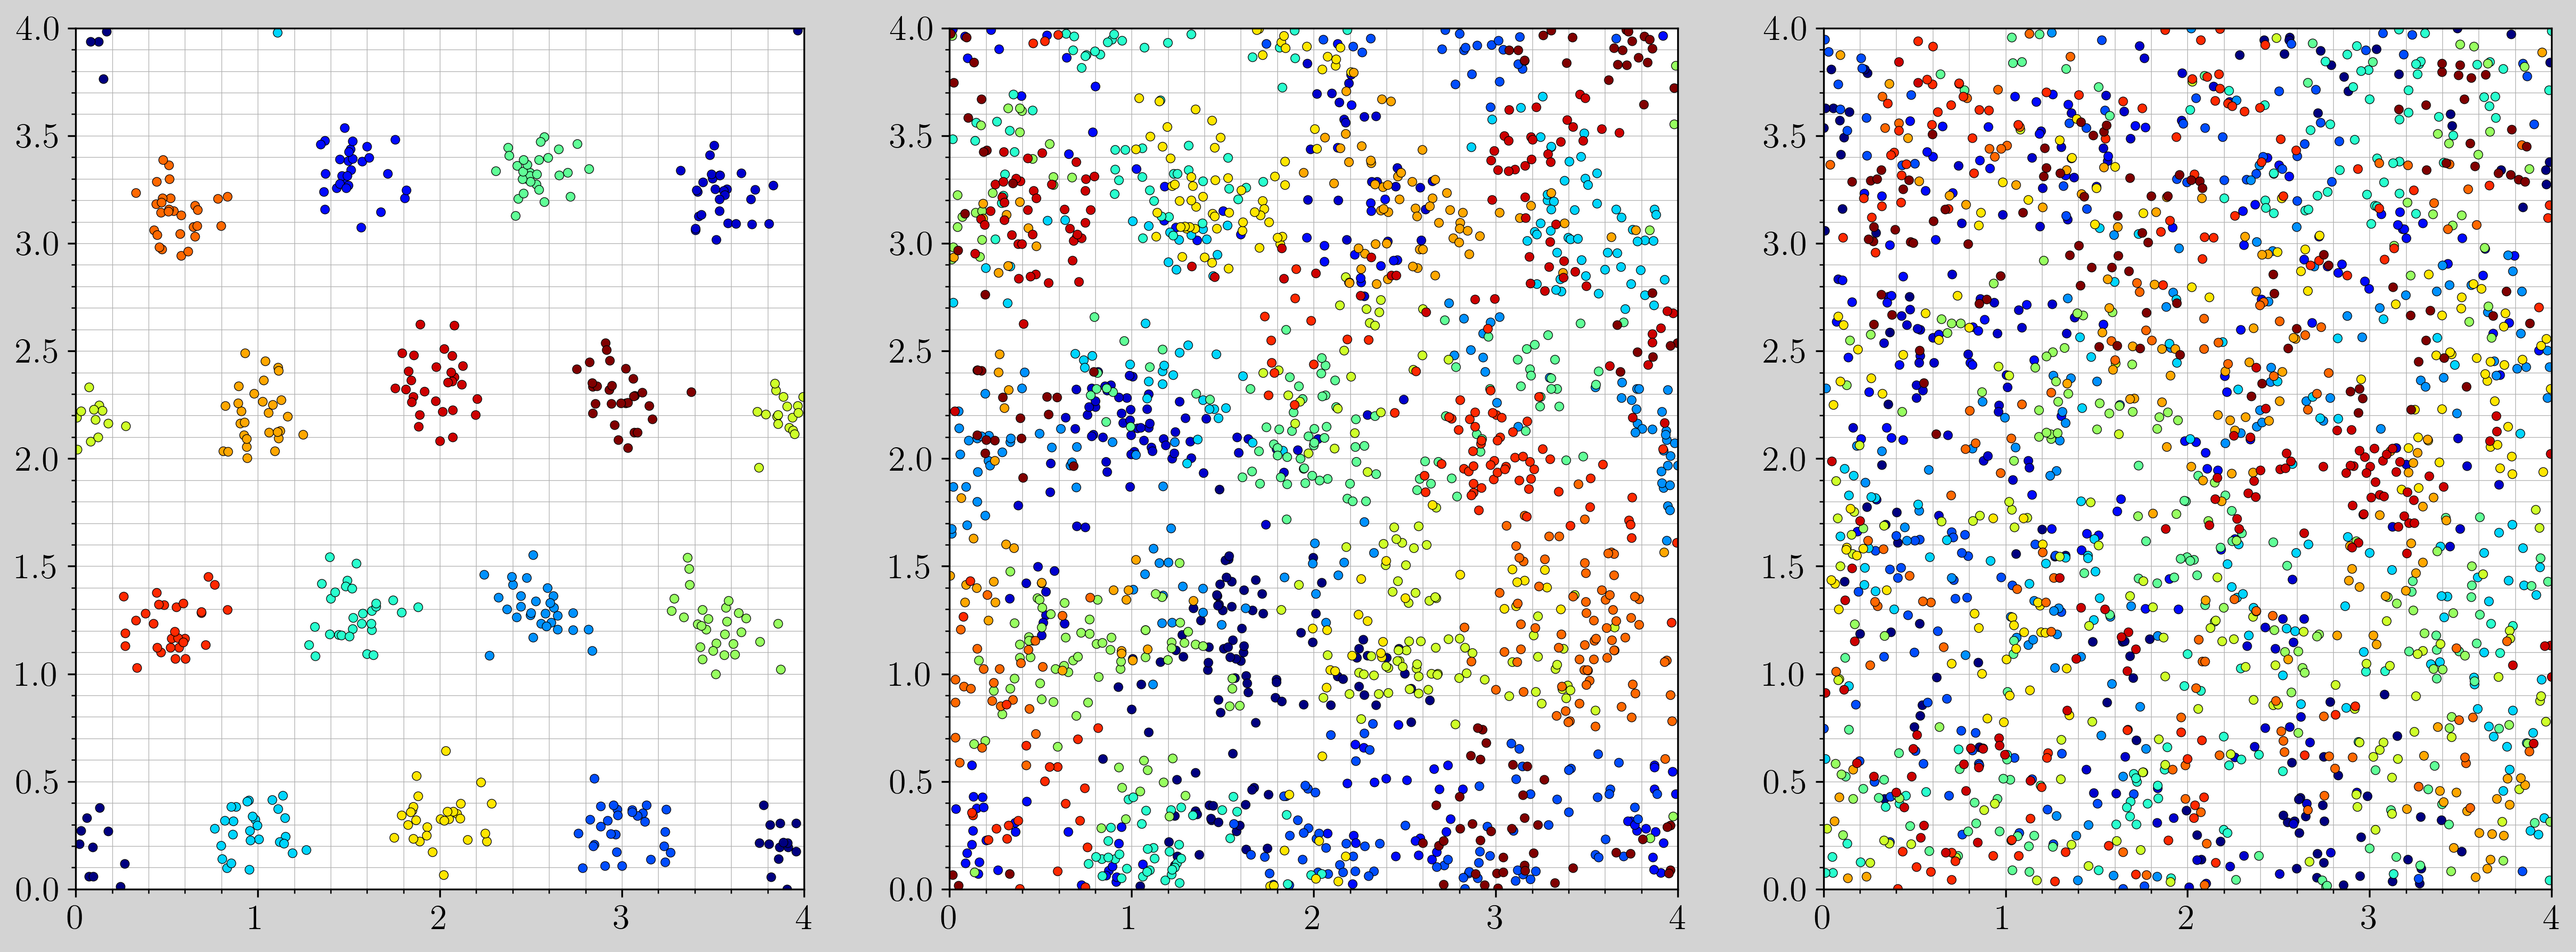
\includegraphics[width=0.95\linewidth]{tarefa-F/posicoes-finais.png}
    \caption{}
    \label{fig:posicoes-finais-f}
\end{figure}


E para finalizar, também foi feito um gráfico da energia desse sistema. Era de se esperar que fosse haver um 
aumentando de energia simplesmente pelo fato de ser um processo de fusão e o gráfico abaixo (\ref{fig:energia-f})
expressa esse fato assim como mostra o quão abrupto é o aumento dessa energia, já que a nossa dinâmica 
de aumento velocidades é instantâneo.

\begin{figure}[h!]
    \centering
    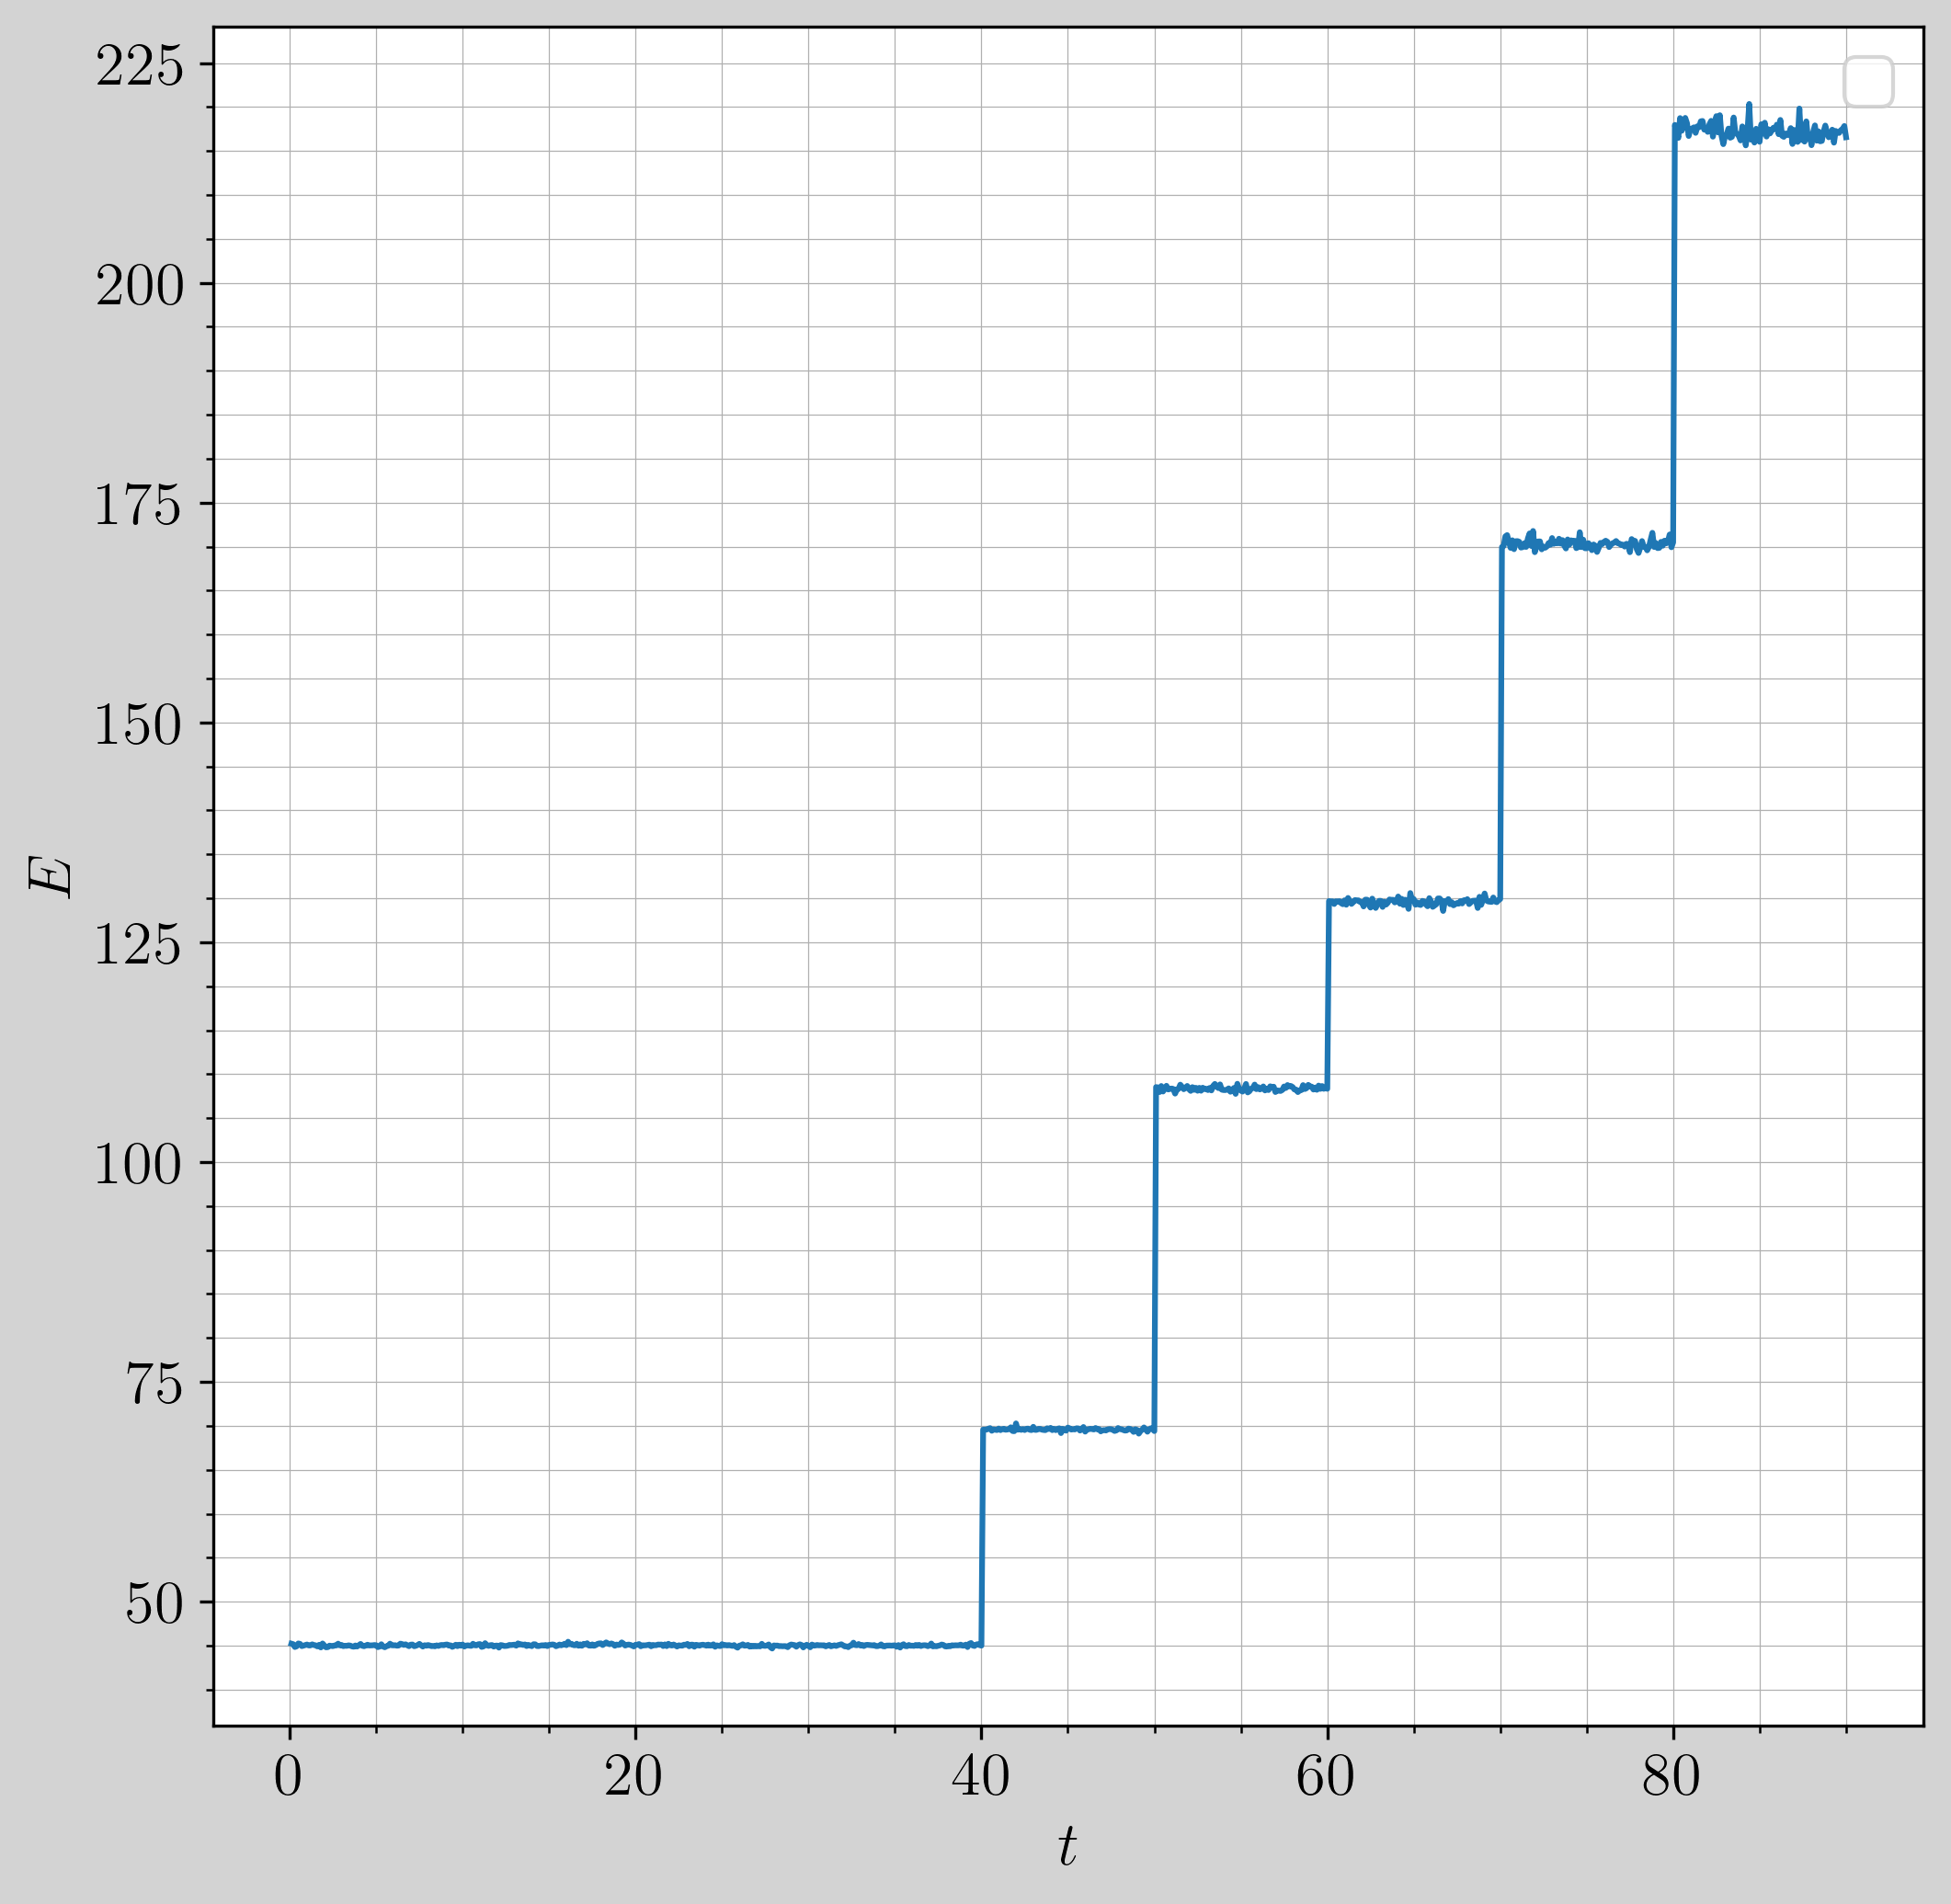
\includegraphics[width=0.4\linewidth]{tarefa-F/energia.png}
    \caption{Energia total a cada tempo.}
    \label{fig:energia-f}
\end{figure}


\clearpage
\subsection{Implementação - Simulação F}
Um detalhe que não consegui explicar sobre essa simulação é que a única forma que consegui fazer a fusão acontecer 
corretamente foi considerando apenas uma das componenentes na (\ref{eq:update_vels}) e não todo vetor. 

\begin{minted}{fortran}
    ! Tarefa F 
    implicit real*8(a-h, o-y)
    parameter (pi = acos(-1.e0))
    dimension r_prev(20, 2)
    dimension r_curr(20, 2)
    dimension r_next(20, 2)
    dimension v(20, 2)
    dimension acc(2)
    dimension r(20, 20)


    ! TAREFA F 
    open(unit=85, file="saidas/tarefa-F/parametros.dat")
    open(unit=86, file="saidas/tarefa-F/posicoes-iniciais.dat")
    open(unit=87, file="saidas/tarefa-F/evolucao-posicoes-1.dat")
    open(unit=88, file="saidas/tarefa-F/evolucao-posicoes-2.dat")
    open(unit=89, file="saidas/tarefa-F/evolucao-posicoes-3.dat")
    open(unit=90, file="saidas/tarefa-F/energia.dat")

    ! Reset variables: 
    r_prev = 0
    r_curr = 0
    r_next = 0
    v = 0

    L = 4
    rL = 4d0
    N = 16

    dt = 5e-3
    v0 = 0.2

    write(85, *) N, L, v0, dt 
    close(85)

    ! Initialize particles 

    n_cols = ceiling(sqrt(N*1d0))
    n_rows = ceiling((N*1d0)/(n_cols*1d0)) 
    
    ! Spacing 1/4 
    x_spacing = L/(1d0*n_cols)
    y_spacing = L/(1d0*n_rows)
    spacing = min(x_spacing, y_spacing)/4.0 
    
    ! Centering in the grid
    x_offset = x_spacing / 2.0 
    y_offset = y_spacing / 2.0
    
    call srand(3512341)

    k = 1 
    do j = 1, n_rows 
          do i = 1, n_cols 
                r_curr(k, 1) = (i-1)*x_spacing+x_offset
                r_curr(k, 2) = (j-1)*y_spacing+y_offset
                
                r_curr(k, 1) = r_curr(k,1)+(rand())*spacing
                r_curr(k, 2) = r_curr(k,2)+(rand())*spacing
                
                theta = 2*pi*rand()
                
                v(k, 1) = v0*cos(theta)
                v(k, 2) = v0*sin(theta)
                
                r_prev(k, 1) = r_curr(k, 1) - v(k, 1) * dt 
                r_prev(k, 2) = r_curr(k, 2) - v(k, 2) * dt 
                k=k+1
          end do 
    end do

    do i = 1, N 
          write(76, *) r_curr(i, 1), r_curr(i, 2)
    end do 
    close(76)

    ! Dynamics 
    do k = 1, 18000 
          t = k * dt 
          acc(1) = 0d0 
          acc(2) = 0d0

          E_k = 0d0
          U = 0d0

          do i = 1, N 
                acc(1) = 0d0 
                acc(2) = 0d0
                do j = 1, N 
                      if(i /= j) then
                           call compute_acc(N,i,j,L,r_curr,acc, r)
                      end if
                end do 
                ! UPDATE POSITIONS
                r_next(i,1) = 2*r_curr(i,1)-r_prev(i,1)+acc(1)*(dt**2)
                r_next(i,2) = 2*r_curr(i,2)-r_prev(i,2)+acc(2)*(dt**2) 

                ! APPLY PBC
                r_next(i,1) = mod(r_next(i,1)+rL, rL)
                r_next(i,2) = mod(r_next(i,2)+rL, rL)

                delta_r_x = delta_pbc(r_next(i,1),r_prev(i,1),L)
                delta_r_y = delta_pbc(r_next(i,2),r_prev(i,2),L)

                ! UPDATE VELOCITIES using adjusted displacements
                v(i, 1) = delta_r_x / (2 * dt)
                v(i, 2) = delta_r_y / (2 * dt)

          end do

          r_prev(:, 1) = r_curr(:, 1)
          r_prev(:, 2) = r_curr(:, 2)
          
          r_curr(:, 1) = r_next(:, 1)
          r_curr(:, 2) = r_next(:, 2)

          if(mod(k, 20) == 0) then 
                if(k > 16000) then
                      ! Liquid end 
                      do i = 1, N
                            write(89,*) k, r_curr(i,1),r_curr(i,2)
                      end do
                else if (k > 10000 .and. k < 12000) then
                      !  Liquit initial
                      do i = 1, N 
                            write(88,*) k, r_curr(i,1),r_curr(i,2)
                      end do
                else if (k > 2600 .and. k < 3200) then 
                      ! Crystal
                      do i = 1, N 
                            write(87,*) k, r_curr(i,1),r_curr(i,2)
                      end do
                end if 

          end if

          ! Increase velocity
          if(mod(k, 2000) == 0 .and. k > 7000) then
                do i = 1, N
                r_prev(i,1)=r_curr(i,1)-(r_curr(i,1)-r_prev(i,1))*1.5
                end do
          end if

          if (mod(k,20) == 0) then
                E = 0d0
                call compute_energy(N, L, v, r_curr, E, r)
                write(90,*) k, E
          end if
    end do 
    close(85)
    close(86)
    close(87)
    close(88)
    close(89)
    close(90)
    end
    ! Submodules for molecular dynamic simulations
    ! Velocity delta 
    function delta_pbc(r_next, r_prev,L)
          implicit real*8(a-h, o-y)
          delta_pbc = r_next - r_prev
          delta_pbc = delta_pbc - L * nint(delta_pbc / L)
    end function delta_pbc

    subroutine initialize_particles(N, L, r_curr,r_prev, v, v0)
          implicit real*8(a-h, o-y)
          dimension r_prev(20, 2)
          dimension r_curr(20, 2)
          dimension v(20, 2)
         
          ! Defining # rows/columns 
          n_cols = ceiling(sqrt(N*1d0))
          n_rows = ceiling((N*1d0)/(n_cols*1d0)) 
          
          ! Spacing 1/4 
          x_spacing = L/(1d0*n_cols)
          y_spacing = L/(1d0*n_rows)
          spacing = min(x_spacing, y_spacing)/4.0 
          
          ! Centering in the grid
          x_offset = x_spacing / 2.0 
          y_offset = y_spacing / 2.0
          call srand(562369)

          k = 1 
          do j = 1, n_rows 
                do i = 1, n_cols 
                      r_curr(k, 1) = (i-1)*x_spacing+x_offset
                      r_curr(k, 2) = (j-1)*y_spacing+y_offset
                      
                      r_curr(k, 1) = r_curr(k,1)+(rand())*spacing
                      r_curr(k, 2) = r_curr(k,2)+(rand())*spacing

                      theta = 2*pi*rand()
                      v(k, 1) = v0*cos(theta)
                      v(k, 2) = v0*sin(theta)
                      
                      r_prev(k, 1) = r_curr(k, 1) - v(k, 1) * dt 
                      r_prev(k, 2) = r_curr(k, 2) - v(k, 2) * dt 
                      k=k+1
                end do 
          end do
    end subroutine initialize_particles

    ! Updates acceleration a = ax, ay 
    ! between particle i and all others
    subroutine compute_acc(N,i,j,L,r_curr,acc, r)
          implicit real*8(a-h, o-y)
          dimension r_curr(20, 2)
          dimension acc(2)
          dimension r(20, 20)
          epsilon = 1e-3

          dx = r_curr(i, 1) - r_curr(j, 1)
          dy = r_curr(i, 2) - r_curr(j, 2)

          dx = dx - L * nint(dx / L)
          dy = dy - L * nint(dy / L)

          r_ij = sqrt(dx**2 + dy**2)
          
          r(i, j) = r_ij 
          r(j, i) = r_ij

          if(r_ij > epsilon .and. r_ij <= 3d0) then 
                F = 24.0 * (2d0/r_ij**13 - 1d0/r_ij**7)
                acc(1) = acc(1) + F * dx / r_ij 
                acc(2) = acc(2) + F * dy / r_ij
          end if 
    end subroutine compute_acc

    subroutine compute_energy(N, L, v, r_curr, E, r)
          implicit real*8(a-h, o-y)
          dimension v(20, 2)
          dimension r_curr(20, 2)
          dimension r(20, 20)
          
          epsilon = 1e-3
          Tk = 0d0
          do i = 1, N
              Tk = Tk + 0.5 * (v(i, 1)**2 + v(i, 2)**2)
          end do
          U = 0d0
          do i = 1, N
            do j = i + 1, N
                r_ij = r(i, j)

                if (r_ij > epsilon .and. r_ij <= 3d0) then
                    U = U + 4 * (r_ij**(-12) - r_ij**(-6))
                end if
            end do
          end do
          E = Tk + U
    end subroutine compute_energy
\end{minted}

\section{Conclusão?} 


Por fim, o arquivo \verb|tests.f| é um compilado de todas simulações desenvolvidas nesse projeto 
e pode ser compilado para rodar todas elas de uma vez. Além disso o script \verb|plots.py| cria todos 
os gráficos e gifs desse trabalho.


\nocite{*}
\printbibliography[title = Referências]
\end{document}
